% !TeX root = ../../../main.tex

\section{The EKO evolution framework}
\label{app:ic/eko}

A crucial ingredient in the derivation of our results
is the determination of the 3FNS intrinsic
charm PDF starting from the 4FNS, which requires the inversion of the matching
conditions implementing the 3FNS to 
the 4FNS transformation.
%
This inversion is not available in the open-source NNPDF
code~\cite{NNPDF:2021uiq} and it is performed here by means of a novel code
for QCD evolution, 
 \textsc{\small EKO} (Evolution Kernel Operators), that we use to take the
 PDF set determined at the reference scale $Q_0$ and evolve it to a
 matching scale $Q_c$ where it is transformed to the 3FNS.
%
Here we provide a brief summary of \textsc{\small
EKO}, some details of the way the direct and inverse matching
conditions are implemented, and some benchmarks between \textsc{\small
EKO} and other existing QCD evolution codes, including the  \textsc{\small
APFEL}~\cite{Bertone:2013vaa} evolution code that is used by the
NNPDF code.
\textsc{\small EKO} is written in \textsc{\small Python} and is available
open source from its \textsc{\small GitHub} repository
\begin{center}
\url{https://github.com/N3PDF/eko}
\end{center}
A more detailed description of the code can be found
in its online documentation
\begin{center}
\url{https://eko.readthedocs.io/en/latest/}
\end{center}
as well as in a dedicated publication~\cite{Candido:2022tld}.

The scale dependence of PDFs in QCD is determined by solving a set
of coupled integro-differential equations (evolution equations) in two
variables $x$ (momentum fraction) and $Q$ (scale) on which PDFs depend.
Two families of approaches are commonly used in order to this purpose.
%
One possibility is to treat the (integral) dependence on $x$ of the
PDFs and evolution kernels by
sampling it on a grid of points.
%
This is the strategy adopted by, among others, the  \textsc{\small APFEL}~\cite{Bertone:2013vaa},
\textsc{\small HOPPET}~\cite{Salam:2008qg},
and \textsc{\small QCDNUM}~\cite{Botje:2010ay} evolution codes.
%
An alternative possibility is to perform an integral transform (Mellin
transform) with
respect to $x$ thereby turning the integro-differential equations into
coupled ordinary differential equations. These can then be solved
analytically, but the integral transform has to be inverted numerically
to arrive at a final result.
%
This approach is adopted by \textsc{\small PEGASUS}~\cite{pegasus} as well as by the
internal PDF evolution code \textsc{\small FastKernel} used in earlier NNPDF analyses
and described in~\cite{DelDebbio:2007ee,Ball:2008by,Ball:2010de}.
%
One limitation of \textsc{\small PEGASUS} is that it requires the analytic
computation of the Mellin transforms of
the PDFs, which is generally not possible, specifically if PDFs are
parametrized as neural networks.
%

This restriction is bypassed in \textsc{\small FastKernel} by transforming only the
evolution kernel (i.e. the evolution operator, solution of differential
equations, evaluated on a given interpolation basis), which can be then
convoluted with the $x$-space PDFs at the input evolution scale $Q_0$.
Following a similar strategy, \textsc{\small EKO}
solves evolution equations in Mellin space and then produces PDF-independent
evolution kernel operators (EKO) which can be convoluted with input 
PDFs.
%
Variable flavor number scheme evolution (VFNS) is implemented in \textsc{\small EKO}, with
the possibility of freely choosing the value of the matching scales
$Q_{h}$ between the $N$-flavor number scheme (NFNS) in which heavy quark $h$
is not included in QCD evolution, and the $(N+1)$-flavor number
scheme in which it is included.
%
Schematically, for evolution between $Q_0$ and $Q_1$ if no matching
scales are crossed $\left(Q_{h}^2 < Q_0^2 , Q_1^2 < Q_{h'}^2\right)$ one has:
\begin{equation}
\label{eq:ic/EKO1}
{\mathbf{f}}^{(n_f)}(Q^2_1)= {\mathbf{E}}^{(n_f)}(Q^2_1\leftarrow Q^2_0) \otimes {\mathbf{f}}^{(n_f)}(Q^2_0) \, ,
\end{equation}
where
${\mathbf{E}}^{(n_f)}$ is the  NFNS \textsc{\small EKO},
and $\otimes$ is the Mellin convolution operation. Note that \textsc{\small EKO}
can perform both ``forward'' ($Q_0< Q_1$)  and ``backward'' ($Q_1< Q_0$)
evolution.
%
Bold quantities indicate either vectors or matrices
in the $(2n_f+1)$-dimensional flavor space.
If instead a single matching scale $Q_h$ is crossed, assuming for definiteness $Q_0< Q_1$,  
$Q_{h'}^2 < Q_0^2 < Q_{h}^2 < Q_1^2 < Q_{h''}^2$,
one has
\begin{equation}
\label{eq:ic/EKO2}
{\mathbf{f}}^{(n_f+1)}(Q^2_1)= \left[ {\mathbf{E}}^{(n_f+1)}(Q^2_1\leftarrow Q_{h}^2)  
{\mathbf{A}}^{(n_f)}(Q_{h}^2) {\mathbf{E}}^{(n_f)}(Q_{h}^2\leftarrow Q^2_0) \right] \otimes {\mathbf{f}}^{(n_f)}(Q^2_0) \, ,
\end{equation}
where $\mathbf{A}^{(n_f)}(Q_{h}^2)$ is the scheme transformation
between the NFNS and (N+1)FNS, given as a perturbatively computable
series expansion in $\alpha_s$. 
%
The quantity in square parenthesis is evaluated in Mellin space and then transformed to $x$-space.
%
This procedure can be  extended to the case in which  more than
one threshold is crossed.
%
Also, the scales $Q_0$ and $Q_1$ can be ordered in any way, because both direct
and inverse scheme transformations are implemented in
\textsc{\small EKO}. Furthermore, the inverse scheme change  is implemented both
perturbatively (i.e.\ as a series expansion in $\alpha_s$ to the same
accuracy as the direct scheme change) or exactly (i.e.\ as the numerical
inverse, completely equivalent to the analytic one within the numeral accuracy
of the rest of the calculation).

If the heavy quark $h$ has no intrinsic component, then below $Q_h$
its PDF is identically zero, and above $Q_h$ it is determined by
$\mathbf{A}^{(n_f)}(Q_{h}^2)$. If it does have an intrinsic
component, then  below $Q_h$ its PDF is scale-independent, but nonzero.
While  \textsc{\small EKO} is currently an NNLO code, on
top of the standard~\cite{pdfnnlo} NNLO scheme change for this work
an N$^3$LO scheme change has been implemented, based on recent higher-order computations
of the relevant operator matrix elements~\cite{Bierenbaum:2009zt,Bierenbaum:2009mv,Ablinger:2010ty,Ablinger:2014vwa,Ablinger:2014uka,Behring:2014eya,Blumlein:2017wxd,Ablinger_2014,Ablinger:2014nga}
and the work of~\cite{zanoli}.

The  \textsc{\small EKO} implementation of QCD evolution has been
benchmarked against the Les Houches PDF evolution
benchmarks~\cite{Dittmar:2005ed,Giele:2002hx} and with
\textsc{\small APFEL} and \textsc{\small PEGASUS},
finding excellent agreement beyond the per-mille level.
%
The implementation of the  matching conditions
has been benchmarked up to N$^3$LO against the independent \textsc{\small Mathematica}-based calculation 
presented in~\cite{zanoli} finding also good agreement.
%
To illustrate some of these benchmarks, Fig.~\ref{fig:ic/EKObench} displays
the absolute and relative difference between \textsc{\small EKO},
\textsc{\small APFEL}, and \textsc{\small PEGASUS}
for NNLO VFNS evolution
carried out
following the settings of~\cite{Dittmar:2005ed,Giele:2002hx}.
%
A toy PDF set at $Q_0=\sqrt{2}$ GeV is evolved up to $Q=100$ GeV
for equal values of the factorization and renormalization scales, $Q_f=Q_r=Q$.
%
We show as representative results those corresponding to
the  total valence quark  $V$ 
and the quark singlet $\Sigma$ distributions.
%
Excellent agreement is found, in particular
with \textsc{\small PEGASUS} which also perform QCD
evolution in Mellin space, with relatively differences
at most at the $\mathcal{O}\left( 10^{-4}\right)$ level.
%
A similar level of agreement is found
for the gluon and for the other quark PDF combinations.

%%%%%%%%%%%%%%%%%%%%%%%%%%%%%%%%%%%%%%%%%%%%%%%%%%%%%%%%%%%%%%%%%%%%%%
\begin{figure}[t]
    \begin{center}
        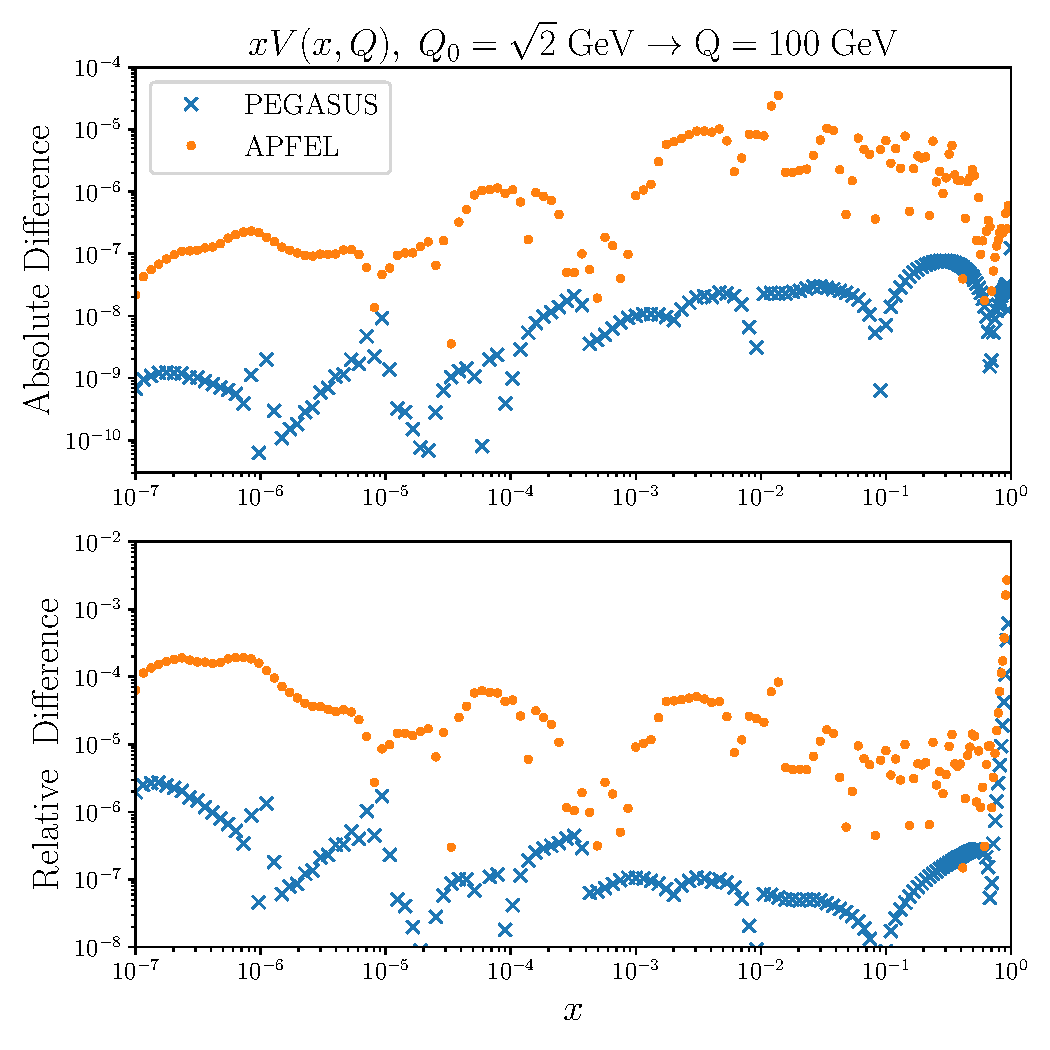
\includegraphics[width=0.47\linewidth]{ch-ic/eko_bench_V.pdf}
        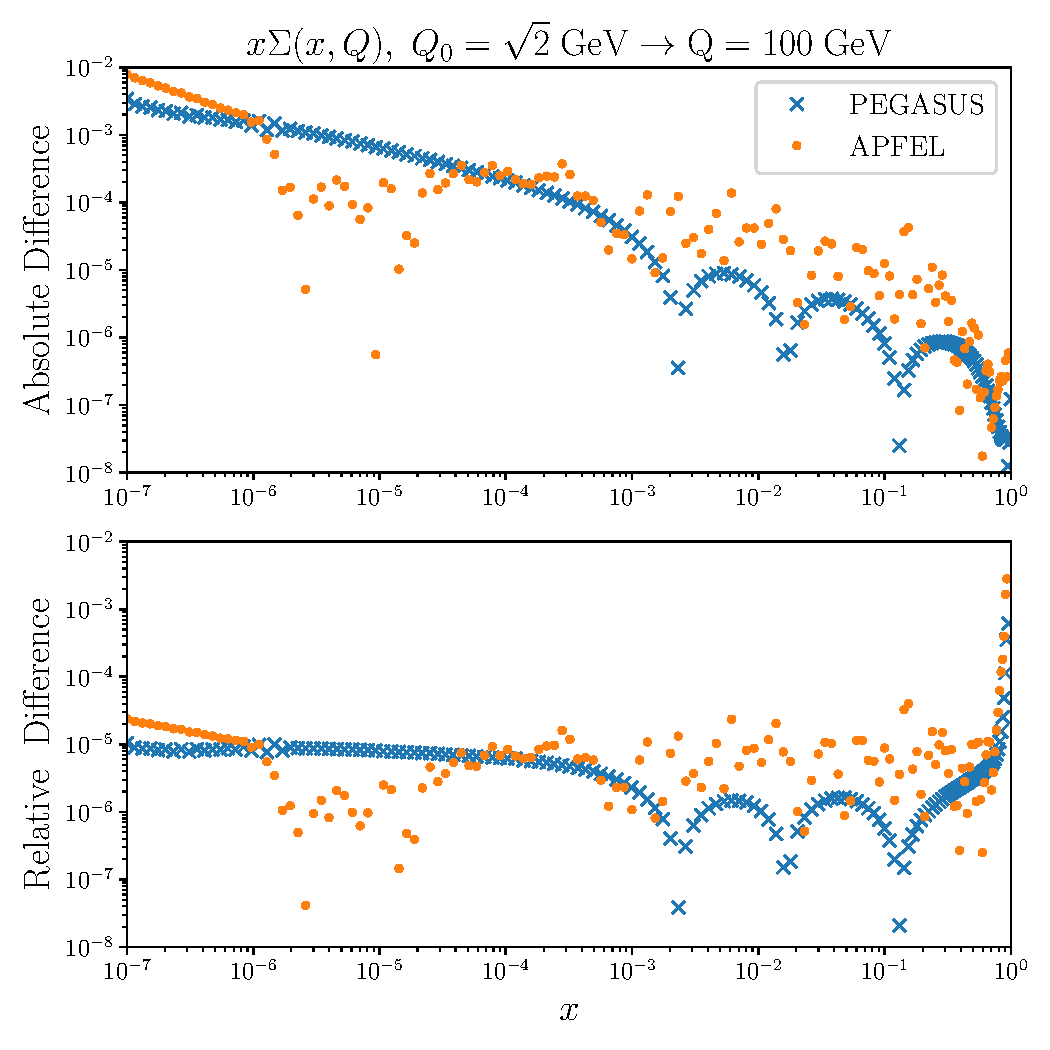
\includegraphics[width=0.47\linewidth]{ch-ic/eko_bench_S.pdf}
        \caption{\small Absolute (upper) and relative (bottom) differences between 
        the outcome of NNLO QCD evolution
        as implemented in
        \textsc{\small EKO} and the
        corresponding results from \textsc{\small APFEL} and \textsc{\small PEGASUS}.
We adopt the settings of the Les Houches PDF evolution benchmarks: we
consider  VFNS evolution from $Q_0=\sqrt{2}$ GeV up to $Q=100$ GeV,
and we show  results for the total valence quark distribution $V$ (left)
and the quark singlet distribution $\Sigma$ (right).
      \label{fig:ic/EKObench} }
    \end{center}
\end{figure}
%%%%%%%%%%%%%%%%%%%%%%%%%%%%%%%%%%%%%%%%%%%%%%%%%%%%%%%%%%%%%%%%%%%%%%



\section{The perturbative charm PDF}
\label{app:ic/consistency}

In the absence of intrinsic charm, the charm PDF is fully determined by
perturbative matching conditions, i.e.\ by the matrix
$\mathbf{A}^{(n_f)}(Q_{c}^2)$ in Eq.~(\ref{eq:ic/EKO2}).
%
We will denote the
charm PDF thus obtained
``perturbative charm PDF'', for short. The PDF
uncertainty on the perturbative charm PDF is directly related to that 
of the light quarks and especially the gluon, and is typically much smaller
than  the  uncertainty on our default charm PDF, that includes
intrinsic charm. Here and in the following we will refer to our final
result, as shown in Fig.~\ref{fig:ic/charm_content_3fns} (right) as ``default''.
%
It should be noticed that the matching conditions for charm are 
nontrivial starting
at NNLO: at NLO the perturbative charm PDF vanishes at threshold.
%
Hence, having implemented in EKO also the N$^3$LO matching conditions,
we are able to assess the MHOU of the perturbative charm at the
matching scale $Q_c$, by comparing
results obtained at the first two nonvanishing perturbative
orders.

As already mentioned, see also Fig.~\ref{fig:ic/Zc}~(top left) in the main manuscript, we have
constructed a PDF set with perturbative charm, in which the full PDF
determination from the global dataset leading to the NNPDF4.0 PDF set
is repeated, but now with the assumption of vanishing intrinsic charm,
i.e.\ with a perturbative charm PDF.
%
This perturbative charm PDF is compared to our default result
in Fig.~\ref{fig:ic/charm_fitted_vs_perturbative_mhous}~(left), where the 4FNS
perturbative 
charm PDF at scale  $Q_c=m_c$ obtained using either NNLO or N$^3$LO
under the assumption of no intrinsic charm are shown, together with
our  result allowing for intrinsic charm.
%
It is clear that while on the one hand, the PDF uncertainty on the
perturbative charm PDF is indeed tiny, on the other
hand the difference between the result for perturbative charm
obtained using NNLO or N$^3$LO matching is large, and in
fact larger at small $x$ than the difference between perturbative charm and our
default (intrinsic) result.

%%%%%%%%%%%%%%%%%%%%%%%%%%%%%%%%%%%%%%%%%%%%%%%%%%%%%%%%%%%%%%%%%%%%%%%%%%
%%%%%%%%%%%%%%%%%%%%%%%%%%%%%%%%%%%%%%%%%%%%%%%%%%%%%%%%%%%%%%%%%%%%%%%%%%
\begin{figure}[h]
  \begin{center}
    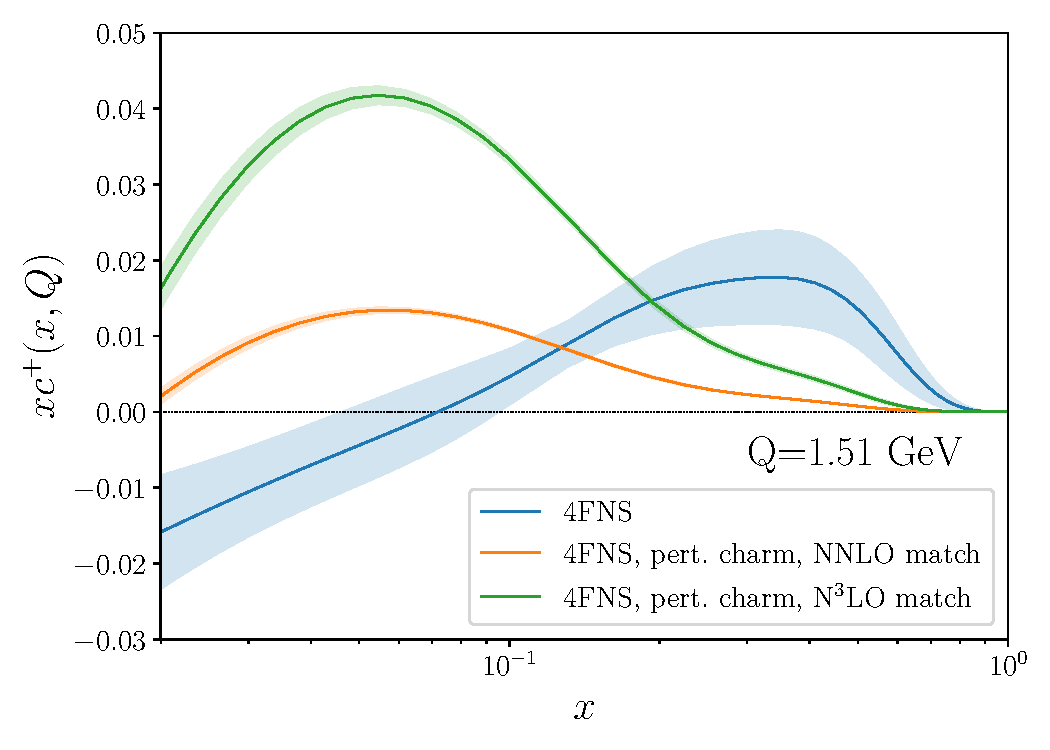
\includegraphics[width=0.49\linewidth]{ch-ic/pch_vs_fitted_forward.pdf}
    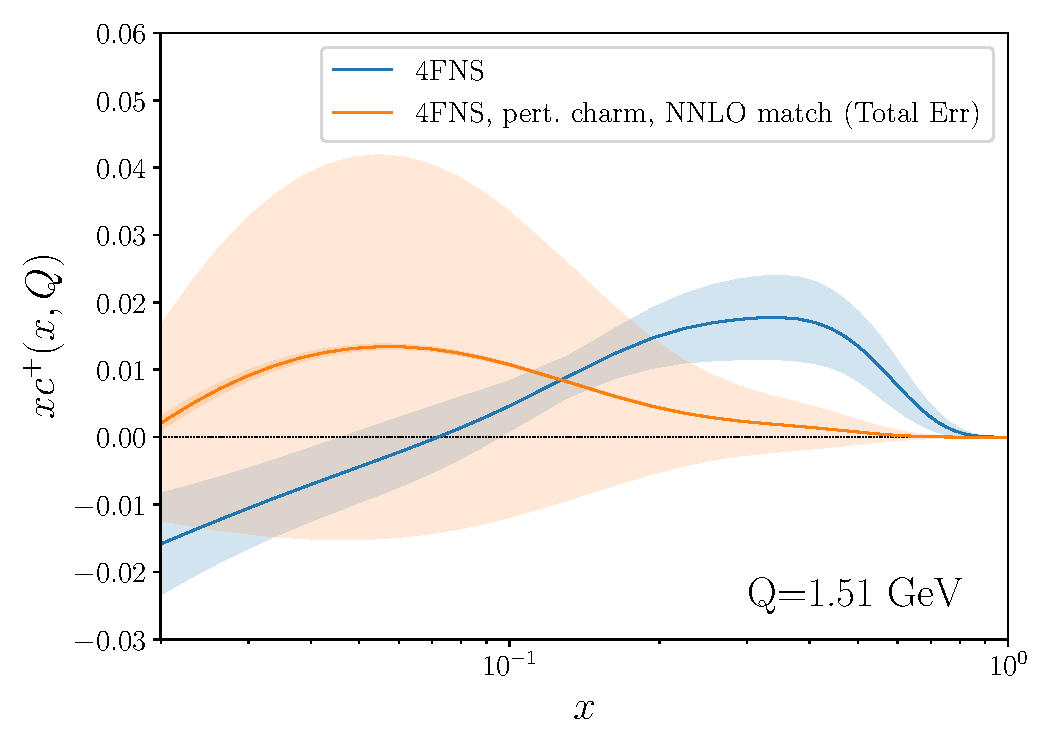
\includegraphics[width=0.49\linewidth]{ch-ic/pch_vs_fitted_forward_MHOU.pdf}
    \caption{\small Left: the perturbative charm PDF at $Q=1.51$~GeV
  obtained from NNLO PDFs using NNLO and N$^3$LO matching
    conditions.
      %
      Right: the NNLO perturbative charm PDF including the MHOU
    computed as the difference between NNLO and N$^3$LO matching.
In both plots our default (intrinsic) charm PDF is also shown for comparison.  
  \label{fig:ic/charm_fitted_vs_perturbative_mhous} }
\end{center}
\end{figure}
%%%%%%%%%%%%%%%%%%%%%%%%%%%%%%%%%%%%%%%%%%%%%%%%%%%%%%%%%%%%%%%%%%%%%%%%
%%%%%%%%%%%%%%%%%%%%%%%%%%%%%%%%%%%%%%%%%%%%%%%%%%%%%%%%%%%%%%%%%%%%%%%%

In the same manner as we used the difference between the results obtained from
inversion of NNLO and N$^3$LO  matching as an estimate of the MHOU on
intrinsic charm, we may use the difference between the 4FNS
 perturbative charm obtained from NNLO and N$^3$LO matching as an
 estimate of the MHOU on perturbative charm at the scale $Q_c$.
 %
 The total uncertainty is found by adding
 this in quadrature to the PDF uncertainty (which however in practice
 is negligible).
%
The result is shown in 
Fig.~\ref{fig:ic/charm_fitted_vs_perturbative_mhous}~(right).
Within this total uncertainty there is now good agreement between our
intrinsic charm result and perturbative charm for all
$x\lsim 0.2$. On the other hand, there is a clear deviation for larger
$x$. We may view the difference between the 4FNS default result
and the 4FNS perturbative  charm as the intrinsic component in the
4FNS, and indeed it is clear from
Fig.~\ref{fig:ic/charm_fitted_vs_perturbative_mhous} that the 4FNS
intrinsic component is sizable and positive at large $x$.
%
This is of course consistent with our main finding that we
only see evidence of intrinsic charm for large $x\gsim 0.2$, while for
smaller $x$ our result for the charm PDF is compatible with zero, as demonstrated by
Fig.~\ref{fig:ic/charm_content_3fns}~(right) in the main manuscript.


\section{Stability of the 4FNS charm PDF}
\label{app:ic/charm_stability_4fns}

The main input to our determination of intrinsic charm is the 4FNS
charm PDF extracted from high-energy data. While this
determination comes with an uncertainty estimate, it is important to
verify that this adequately reflects the various sources
of uncertainty, and that there are no further sources of uncertainty
that may be unaccounted for.
%
To this purpose, here we assess the
stability of our results first, upon the choice of underlying dataset,
next upon changes in methodology, and finally, upon variation of
standard model parameters.
%
In each case we verify stability upon the
most important possible source of instability: respectively, the use
of collider vs.\ fixed target and deep-inelastic vs.\ hadronic data
(dataset); the choice of parametrization basis (methodology); and the
value of the charm quark mass (standard model parameters).
%
As a final consistency check, we compare our result with that which we
would have obtained by using the same input dataset, but the previous
NNPDF3.1 fitting methodology.
%
Because we
are interested in intrinsic charm, in all comparisons we focus on
the large-$x$ region in which the intrinsic valence-like peak is found.
%
In this section, the 4FNS
charm PDF is displayed at the scale $Q = 1.65$ GeV so that
results for all fit variants, including
those with with different $m_c$ values, can be shown at a common scale.

\paragraph{Dependence on the choice of dataset.}
%
We now study the stability of the  4FNS charm determination upon
variation of the
underlying data, which also allows us to
identify the datasets or groups of processes that provide
the leading constraints on intrinsic charm.
%
To this purpose, we have repeated our PDF
determination using a  variety of subsets of the global dataset used for
our default determination. Results are shown in
Fig.~\ref{fig:ic/charm_dataset_dep}, where we compare the result using
the 
baseline dataset to determinations performed by adding to the baseline
the  EMC charm
structure function data (already discussed in the main text); by only
including  DIS data; by only including collider data (HERA,
Tevatron and LHC); and by removing the LHCb  $W$ and $Z$ production data.

%%%%%%%%%%%%%%%%%%%%%%%%%%%%%%%%%%%%%%%%%%%%%%%%%%%%%%%%%%%%%%%%%%%
\begin{figure}[t!]
  \begin{center}
    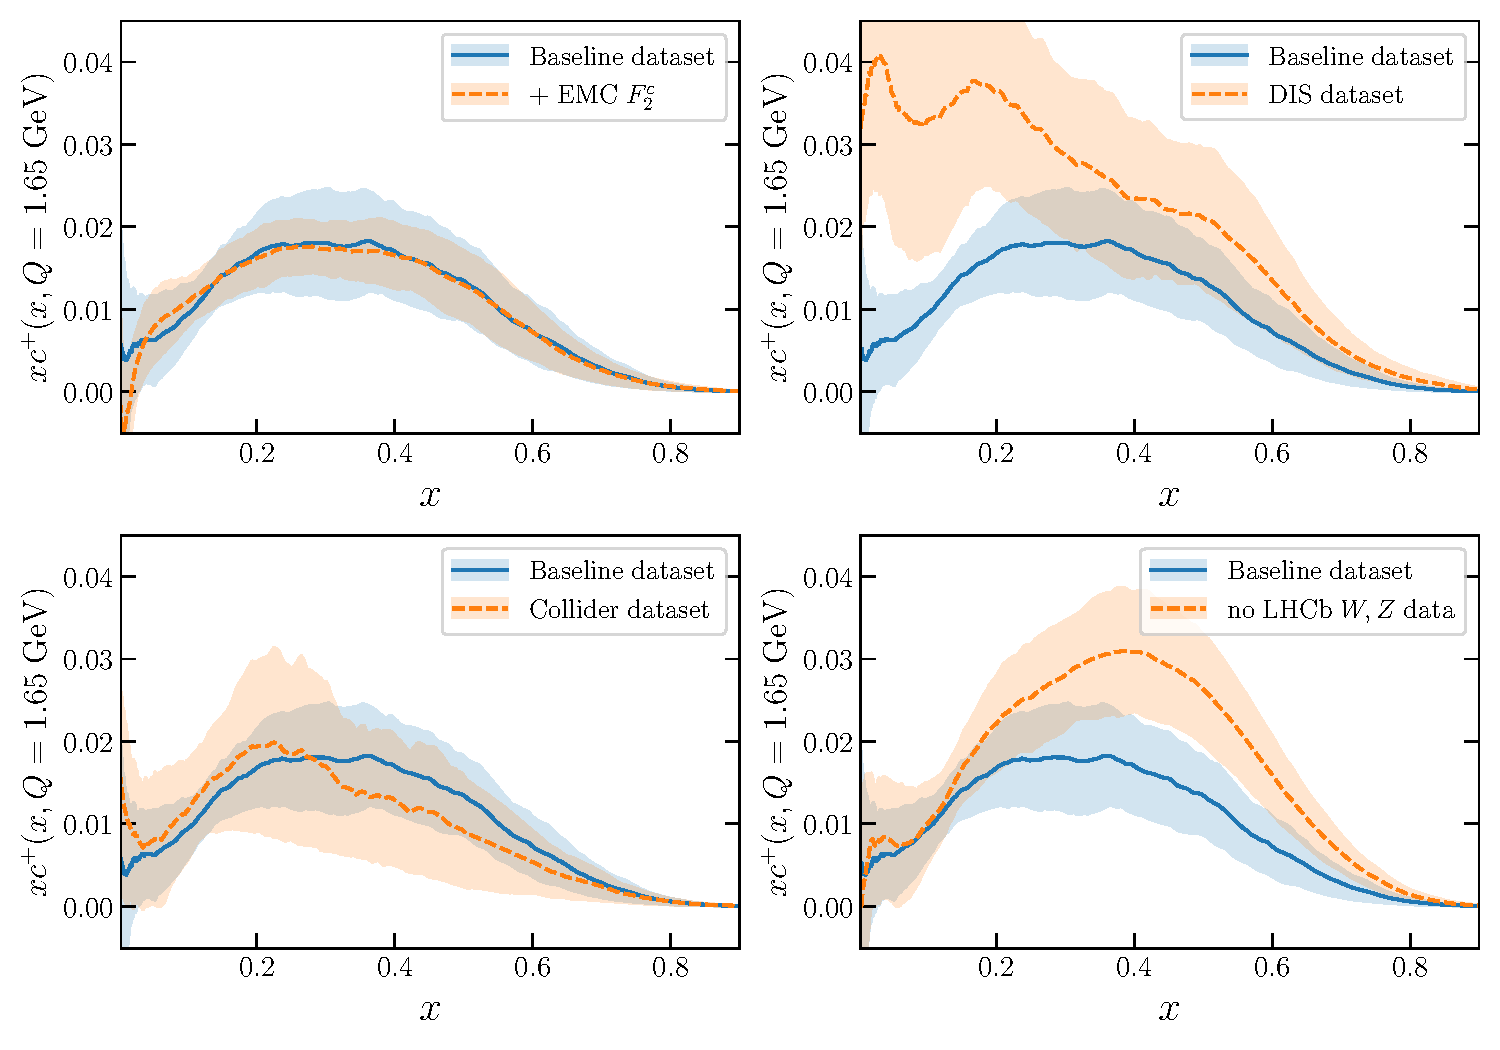
\includegraphics[width=0.99\linewidth]{ch-ic/pdfplot-abscharm-dataset_dep.pdf}
    \caption{\small The dependence of the 4FNS charm PDF at $Q=1.65$ GeV on
      the input dataset.
      %
      We compare the
    baseline result with that obtained by also including 
      EMC $F_2^c$ data (top left), only including DIS data (top
    right), only including collider data (bottom left) and removing
    LHCb gauge boson production data (bottom right). 
  \label{fig:ic/charm_dataset_dep} }
\end{center}
\end{figure}
%%%%%%%%%%%%%%%%%%%%%%%%%%%%%%%%%%%%%%%%%%%%%%%%%%%%%%%%%%%%%%%%%%%%%%

As already noted in the main  text in the case of the 3FNS
result, we find that the extra information provided by the  EMC
$F_2^c$ data is subdominant in comparison to that from the global
dataset. The result is stable and only a moderate
uncertainty reduction at the peak is observed. It is interesting to
contrast this with the previous NNPDF study~\cite{Ball:2016neh}, in
which the global fit provided only very loose constraints on the charm
PDF, which was then determined mostly by the EMC data.
%
Indeed, a DIS-only fit (for which most data were already available at the time
of the previous determination) determines charm with very large
uncertainties. On the other hand, both the central value and
uncertainty found in the collider-only fit are quite similar to the
baseline result.
%
This shows that the dominant constraint is now coming from
collider, and specifically hadron collider data (indeed, as we have
seen constraints from DIS data are quite loose). Among these, LHCb
data (which are taken at large rapidity and thus impact PDFs at large
and small $x$) are especially important, as demonstrated by the
increase in uncertainty when they are removed.

In all these determinations, the charm
PDF at $x\simeq 0.4$ remains consistently nonzero and positive, thus
emphasizing the stability of our results.

\paragraph{Dependence on the parametrization basis.}
%
Among the various methodological choices, a possibly critical one is
the choice of basis functions. Specifically, in our default analysis,
the output of the neural network does not provide the individual
quark flavor and antiflavor PDFs, but rather linear combinations
corresponding to the so-called evolution
basis~\cite{Ball:2021leu}. Indeed, our charm PDF is given in
Eq.~(\ref{eq:ic/fitted_charm_param})  as the linear combination of the
two basis PDFs $\Sigma$ and $T_{15}$.
One may thus ask whether this choice may influence the final results
for individual quark flavors, specifically charm.
Given that physical results are basis
independent, the outcome of a PDF determination should not depend
on the basis choice.

In order to check this, we have repeated the PDF determination, but
now using the flavor basis, see Sect.~3.1 of~\cite{Ball:2021leu}, in which
each of the  neural network output neurons now correspond to individual quark
flavors, so in particular,
instead of Eq.~(\ref{eq:ic/fitted_charm_param}),  one has
\begin{equation}
\label{eq:ic/fitted_charm_param_flavour}
xc^+(x,Q_0;{\boldsymbol \theta}) =
 (1-x)^{\beta_{c^+}} \textrm{ NN}_{c^+}(x,{\boldsymbol \theta}) \, ,
\end{equation}
where $\textrm{ NN}_{c^+}(x,{\boldsymbol \theta})$
indicates the value of the output neuron associated to the charm PDF $c^+$.
%
The 4FNS charm PDFs determined using either basis are compared 
in Fig.~\ref{fig:ic/charm_basisdep}  at $Q=1.65$ GeV.
%
We find excellent consistency, and in particular 
the valence-like structure at high-$x$ is independent of the choice
of parametrization basis.

%%%%%%%%%%%%%%%%%%%%%%%%%%%%%%%%%%%%%%%%%%%%%%%%%%%%%%%%%%%%%%%%%%%
\begin{figure}[t!]
  \begin{center}
    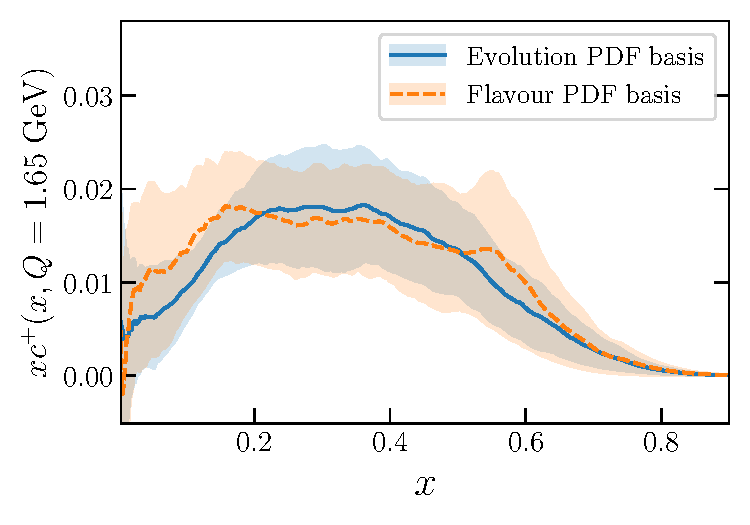
\includegraphics[width=0.60\linewidth]{ch-ic/pdfplot-abscharm-basisdep.pdf}
    \caption{\small The default 4FNS charm PDF at $Q=1.65$ GeV
    compared to a result obtained by parametrizing PDFs in the flavor
    basis instead of the evolution basis. 
  \label{fig:ic/charm_basisdep} }
\end{center}
\end{figure}
%%%%%%%%%%%%%%%%%%%%%%%%%%%%%%%%%%%%%%%%%%%%%%%%%%%%%%%%%%%%%%%%%%%%%%

\paragraph{Dependence on the charm mass.}
%
The kinematic threshold for producing charm perturbatively depends on
the value of the charm mass. Therefore the perturbative contribution
to the 4FNS charm PDF, and thus the whole charm PDF if one assumes
perturbative charm, depends strongly on the value of the charm
mass.
On the other hand, the intrinsic charm PDF is of nonperturbative
origin, so it should be essentially independent of the numerical value of the
charm mass that is used in  perturbative computations employed in  its 
determination (though it will of course depend on the true underlying 
physical value of the charm mass).

In order to study this mass dependence, we have repeated our determination using different values for the charm mass.
The definition of the charm mass which is relevant for kinematic
thresholds is the pole mass, for which we adopt the value recommended
by the Higgs cross-section working group~\cite{deFlorian:2016spz}
based on the study of~\cite{Bauer:2004ve}, namely
 $m_c = 1.51 \pm 0.13$~GeV. 
%
Results are shown in Fig.~\ref{fig:ic/charm_fitted_mcdep}, where
our default charm PDF determination with  $m_c = 1.51$~GeV is
repeated with $m_c=1.38$~GeV and
$m_c=1.64$~GeV.
%
In order to understand these results note that this is
the 4FNS PDF, so it includes 
both a nonperturbative and a perturbative component. The latter is
strongly dependent on the charm mass, but of course the data
correspond to the unique true value of the mass and the mass
dependence of the perturbative component is present only due to our
ignorance of the actual true value. When determining the PDF from the
data, as we do, we expect this spurious dependence to be to some extent
reabsorbed into the fitted PDF. So we expect results to display a
moderate dependence on the charm mass --- full independence should
hold for the intrinsic (3FNS) PDF and will be investigated in
SI Sect.~\ref{app:ic/charm_stability_3fns}. 

In Fig.~\ref{fig:ic/charm_pert_mcdep} the same result is shown, but now
for the perturbative charm PDF discussed in
SI Sect.~\ref{app:ic/consistency},  so the charm PDF is of
purely perturbative origin and fully determined by the strongly
mass-dependent matching condition. This dependence is clearly seen in
the plots. Furthermore, comparison with
Fig.~\ref{fig:ic/charm_fitted_mcdep} shows that indeed this spurious
dependence is partly reabsorbed in the fit when the charm PDF is
determined from the data, so that  the residual mass dependence is moderate.
In particular, the large-$x$ valence peak, which is dominated by the
intrinsic component, is very stable.

%%%%%%%%%%%%%%%%%%%%%%%%%%%%%%%%%%%%%%%%%%%%%%%%%%%%%%%%%%%%%%%%%%%
\begin{figure}[t]
  \begin{center}
    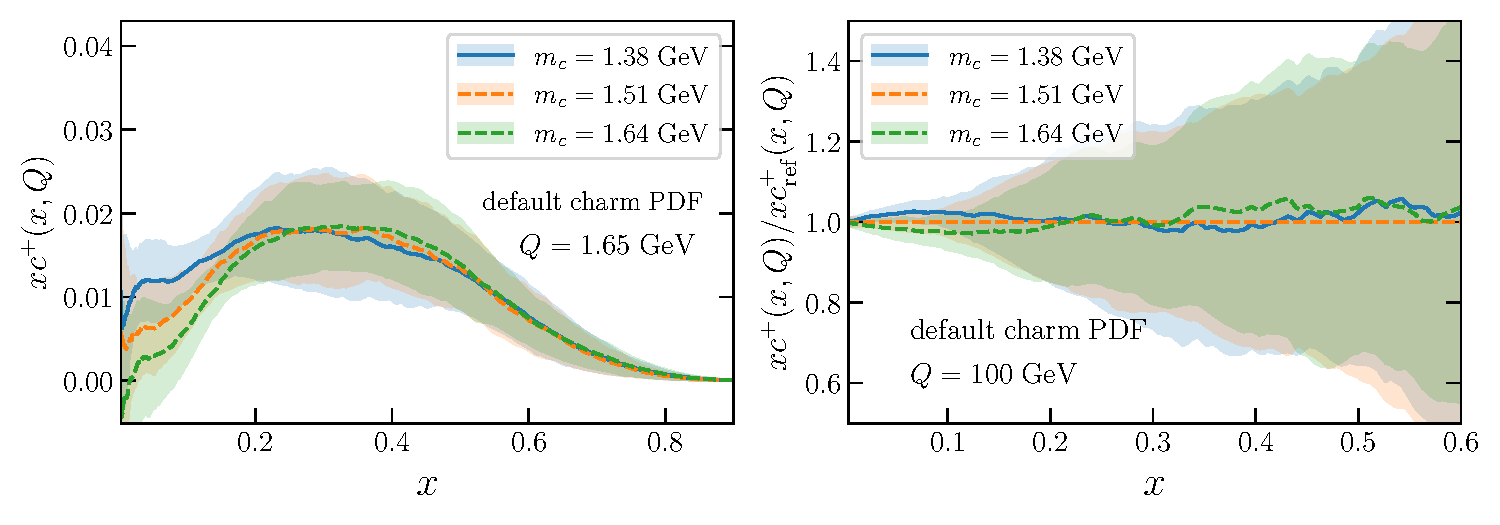
\includegraphics[width=0.99\linewidth]{ch-ic/pdfplot-abscharm-mcdep.pdf}
    \caption{\small The 4FNS charm PDF determined
    using three different values of the charm mass. The absolute
    result (left) is shown at $Q=1.65$ GeV, while the ratio to the 
       default value
       $m_c=1.51$~GeV (right) used elsewhere in this paper is shown at $Q=100$ GeV.
   \label{fig:ic/charm_fitted_mcdep} }
\end{center}
\end{figure}
%%%%%%%%%%%%%%%%%%%%%%%%%%%%%%%%%%%%%%%%%%%%%%%%%%%%%%%%%%%%%%%%%

%%%%%%%%%%%%%%%%%%%%%%%%%%%%%%%%%%%%%%%%%%%%%%%%%%%%%%%%%%%%%%%%%%%
\begin{figure}[t]
  \begin{center}
    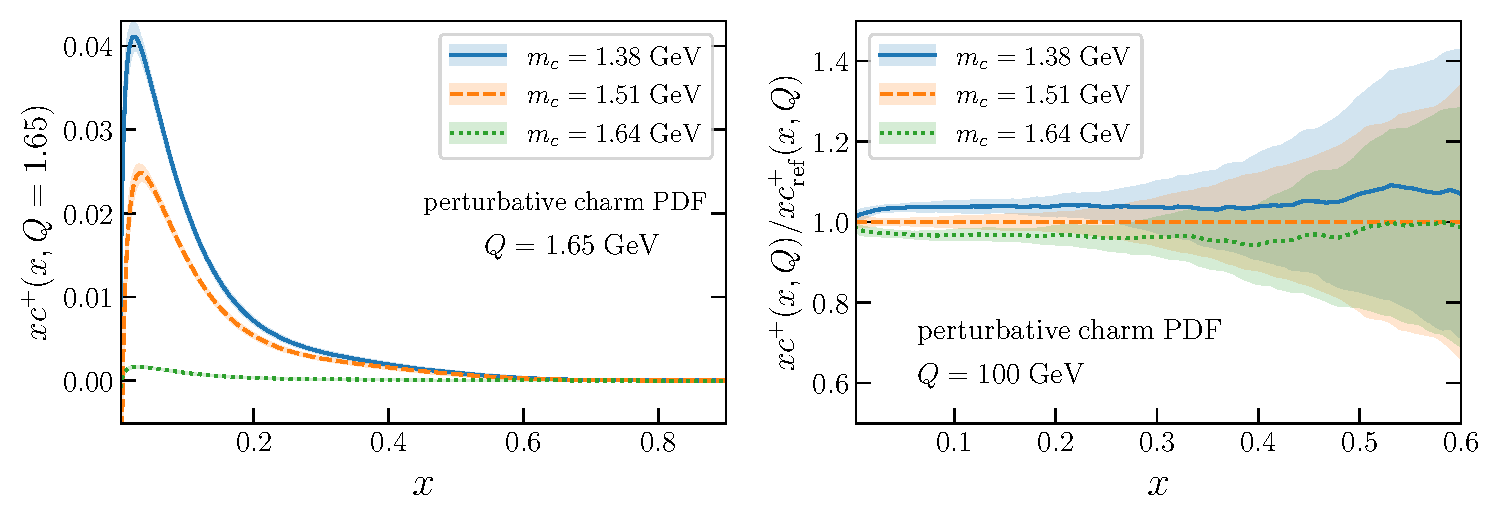
\includegraphics[width=0.99\linewidth]{ch-ic/pdfplot-abscharm-mcdep-highQ.pdf}
    \caption{\small The same as Fig.~\ref{fig:ic/charm_fitted_mcdep} but now
    for the perturbative charm PDF.
  \label{fig:ic/charm_pert_mcdep} }
\end{center}
\end{figure}
%%%%%%%%%%%%%%%%%%%%%%%%%%%%%%%%%%%%%%%%%%%%%%%%%%%%%%%%%%%%%%%%%



  \paragraph{Comparison with NNPDF3.1.}
  %
  Fig.~\ref{fig:ic/pdfplot-abscharm-40-vs-31meth} compares
  the baseline determination of the 4FNS charm PDF based
  on NNPDF4.0 with that obtained
  from the same input dataset but using instead
  the NNPDF3.1 fitting methodology and related settings such those related to positivity
  and integrability.
  %
  Results are fully consistent between the two methodologies, with our default
  determination exhibiting reduced uncertainties due to
  the various improvements implemented
  in the NNPDF4.0 analysis framework.
  
%%%%%%%%%%%%%%%%%%%%%%%%%%%%%%%%%%%%%%%%%%%%%%%%%%%%%%%%%%%%%%%%%%%
\begin{figure}[t]
  \begin{center}
    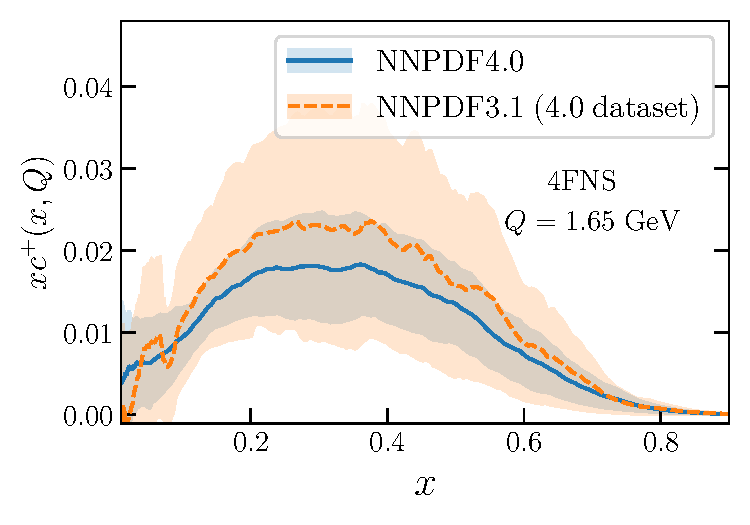
\includegraphics[width=0.65\linewidth]{ch-ic/pdfplot-abscharm-40-vs-31meth.pdf}
    \caption{\small Same as Fig.~\ref{fig:ic/charm_basisdep}, comparing
      the baseline determination of the 4FNS charm PDF, based
      on NNPDF4.0, with that obtained
      from the same dataset using the NNPDF3.1 fitting methodology.
  \label{fig:ic/pdfplot-abscharm-40-vs-31meth} }
\end{center}
\end{figure}
%%%%%%%%%%%%%%%%%%%%%%%%%%%%%%%%%%%%%%%%%%%%%%%%%%%%%%%%%%%%%%%%%




\section{Stability of the 3FNS charm calculation}
\label{app:ic/charm_stability_3fns}

We now repeat the stability and uncertainty
study of the previous section, but for our final
result, namely the intrinsic charm PDF. The main difference to be kept
in mind is that the uncertainty now also includes the dominant MHOU,
due to the matching condition required in order to determine the 3FNS
PDF from the 4FNS result. In order to get a complete picture, we now
add a further set of dataset variations.

\paragraph{Dependence on the input dataset.}
%
Fig.~\ref{fig:ic/charm_dataset_dep_nf3} displays the dataset variations shown in
Fig.~\ref{fig:ic/charm_dataset_dep}, now for the intrinsic (3FNS) charm
PDF, but with the total uncertainty now being the sum in quadrature of
the PDF and MHO uncertainties, with the latter determined as the difference between
results obtained using NNLO and N$^3$LO matching.
%
Additionally, we also performed a few extra  dataset
variations: a fit without any $W, Z$ production data from ATLAS and CMS,
a fit without jet data, a fit without $Z$ $p_T$ measurements, and a fit without
HERA structure function data.
%
Note that the collider-only dataset includes both HERA electron-proton
collider data and Tevatron and LHC hadron collider data, but not
fixed-target deep-inelastic scattering and Drell-Yan production data.


Results are qualitatively very similar to those seen in the 4FNS, a
consequence of the fact that we are focusing on the large-$x$ region where the
effect of the matching is moderate, though now the presence of a
valence-like peak in all determinations is even clearer, specifically
for the DIS-only fit where it was less pronounced in the 4FNS.
%
 Note however that the DIS-only determination
  exhibits larger uncertainties
  (up to factor 2) and point-by-point fluctuations,
  and is dominated by relatively old fixed-target measurements.
%
Comparison of all the dataset variations shows that, in terms of their
impact on intrinsic charm,
hadron collider data are generally more important
that deep-inelastic data, that among the former the
LHCb inclusive $W,Z$ data are playing a dominant role,
and that jet observables also play a non-negligible role.

It should be stressed that the agreement between results found using
DIS data and hadron collider data is highly nontrivial, since in the region
relevant for intrinsic charm these determinations are based on disjoint datasets
and are  affected by
very different theoretical and experimental uncertainties:
in particular, potential higher-twist
effects in the DIS observables are highly suppressed for collider observables.
%
 this respect, a DIS-only determination of intrinsic charm
  is potentially affected by sources of theory uncertainties, such as higher twists,
which are not accounted for in global PDF determinations.

%%%%%%%%%%%%%%%%%%%%%%%%%%%%%%%%%%%%%%%%%%%%%%%%%%%%%%%%%%%%%%%%%%%
\begin{figure}[h]
  \begin{center}
    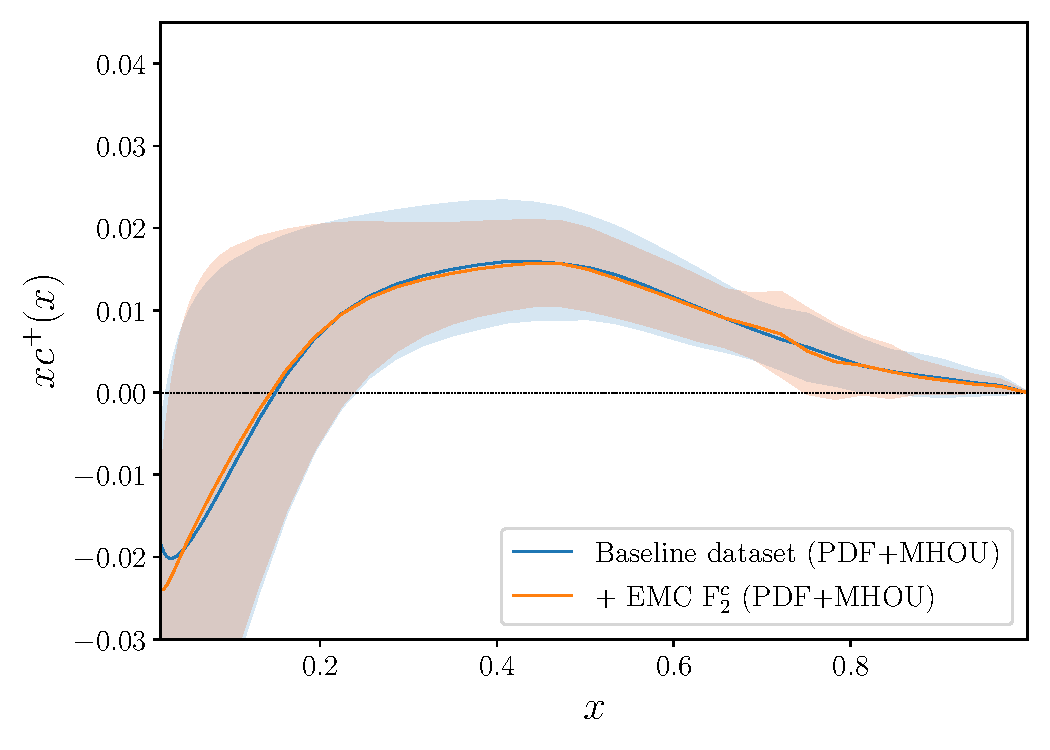
\includegraphics[width=0.49\linewidth]{ch-ic/EMC_Quad_MHOU.pdf}
    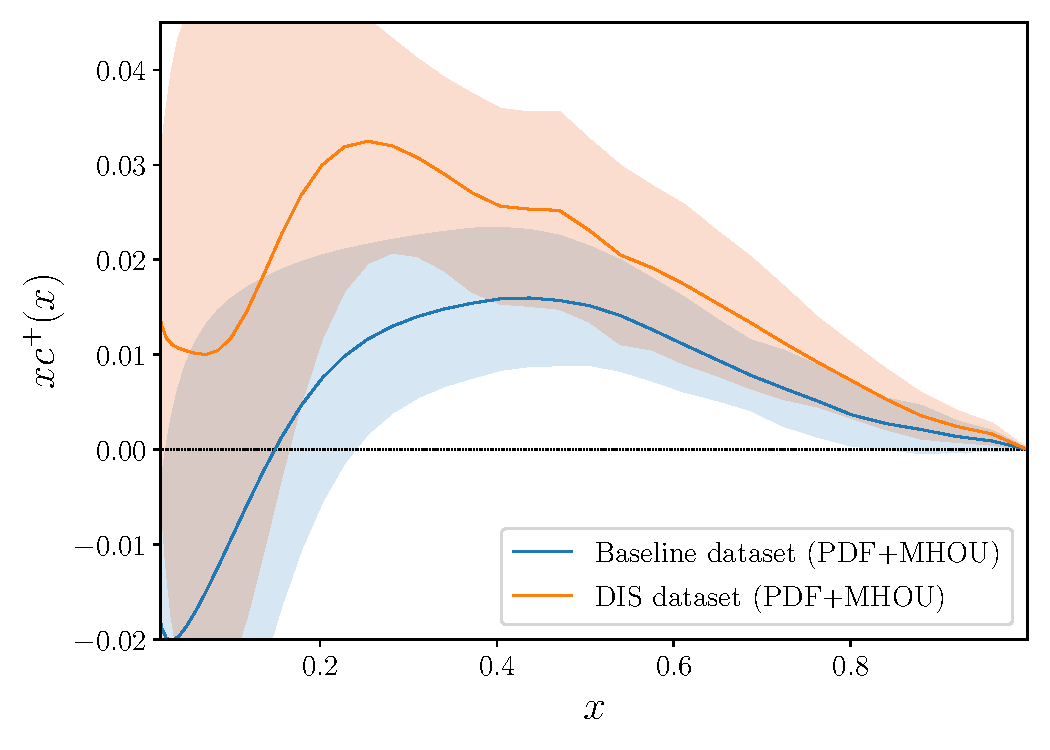
\includegraphics[width=0.49\linewidth]{ch-ic/DIS_only_Quad_MHOU.pdf}
    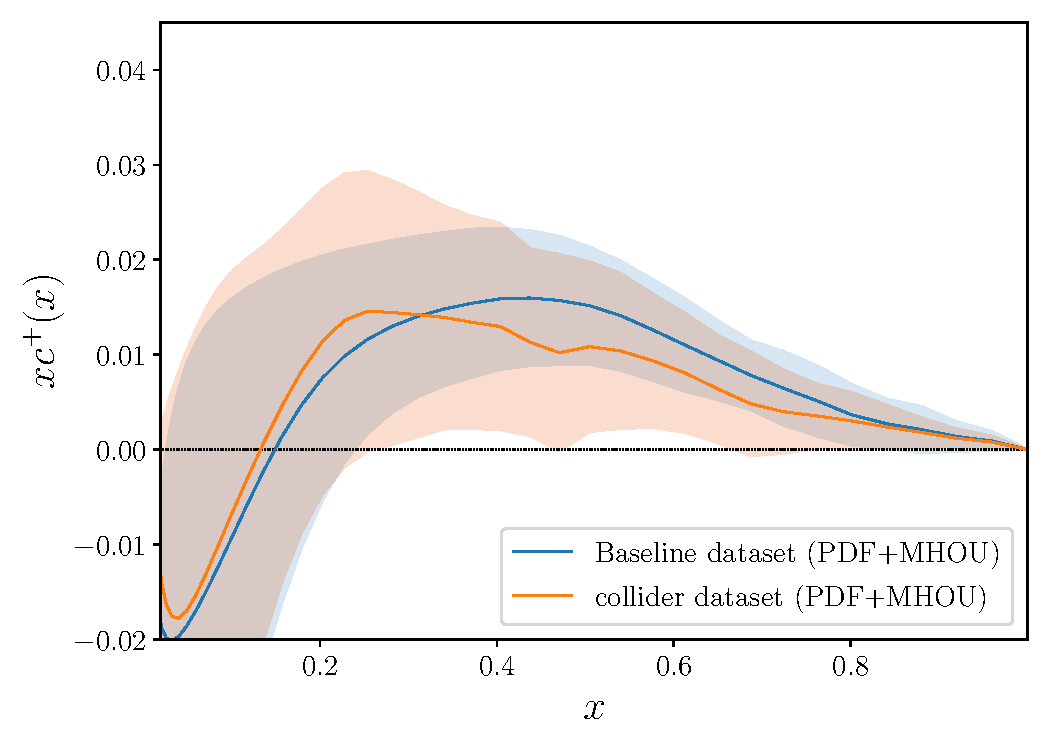
\includegraphics[width=0.49\linewidth]{ch-ic/collider_only_Quad_MHOU.pdf}
    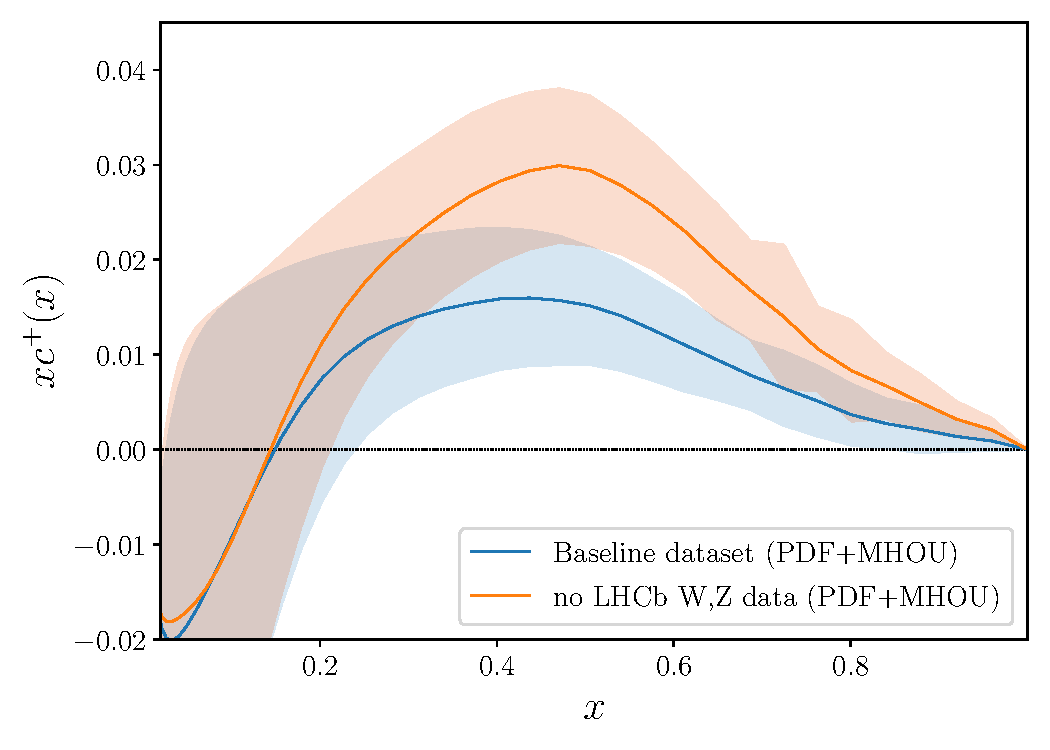
\includegraphics[width=0.49\linewidth]{ch-ic/noLHCb_Quad_MHOU.pdf}
    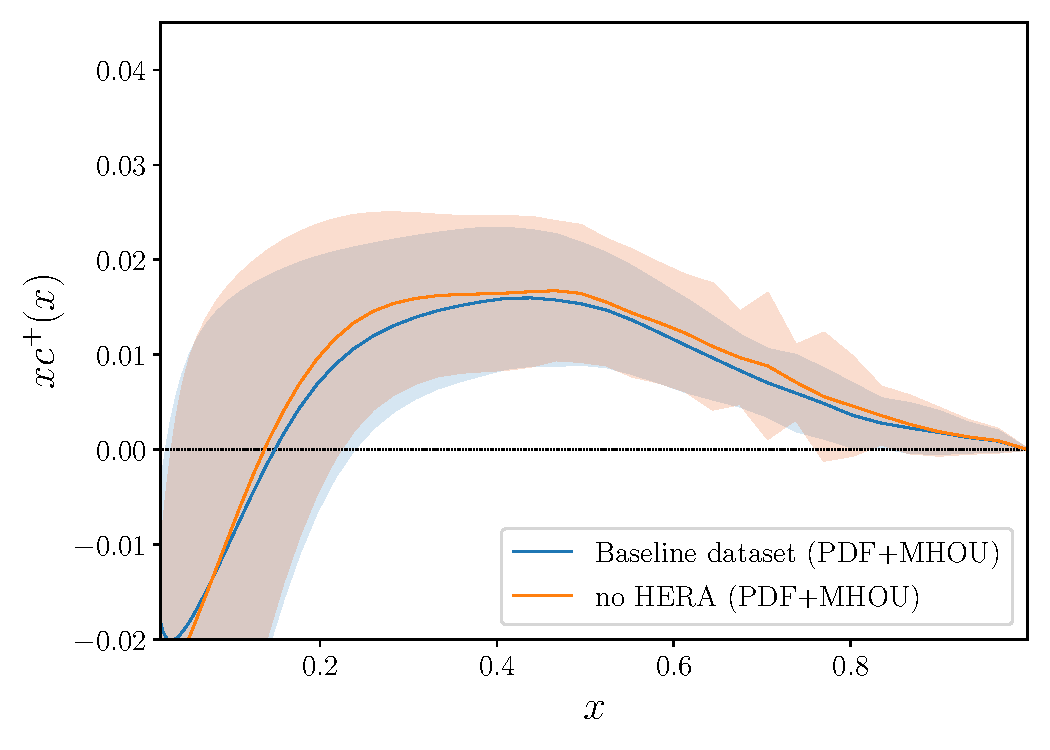
\includegraphics[width=0.49\linewidth]{ch-ic/noHERA_Quad_MHOU.pdf}
    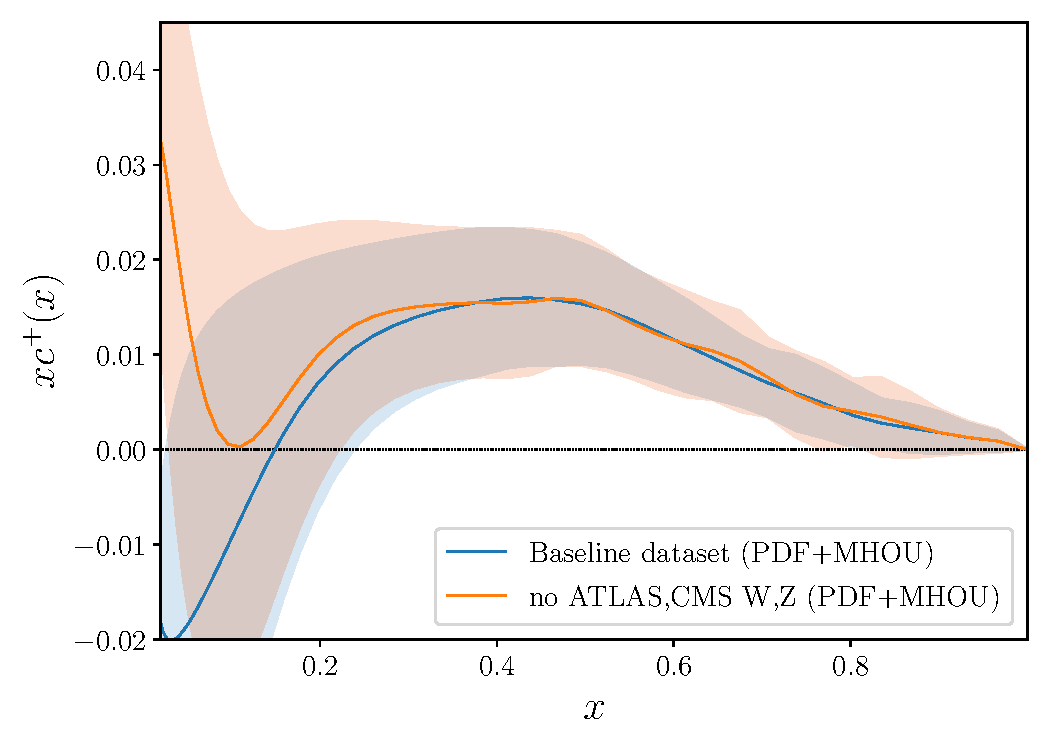
\includegraphics[width=0.49\linewidth]{ch-ic/noATLASCMSDY_Quad_MHOU.pdf}
    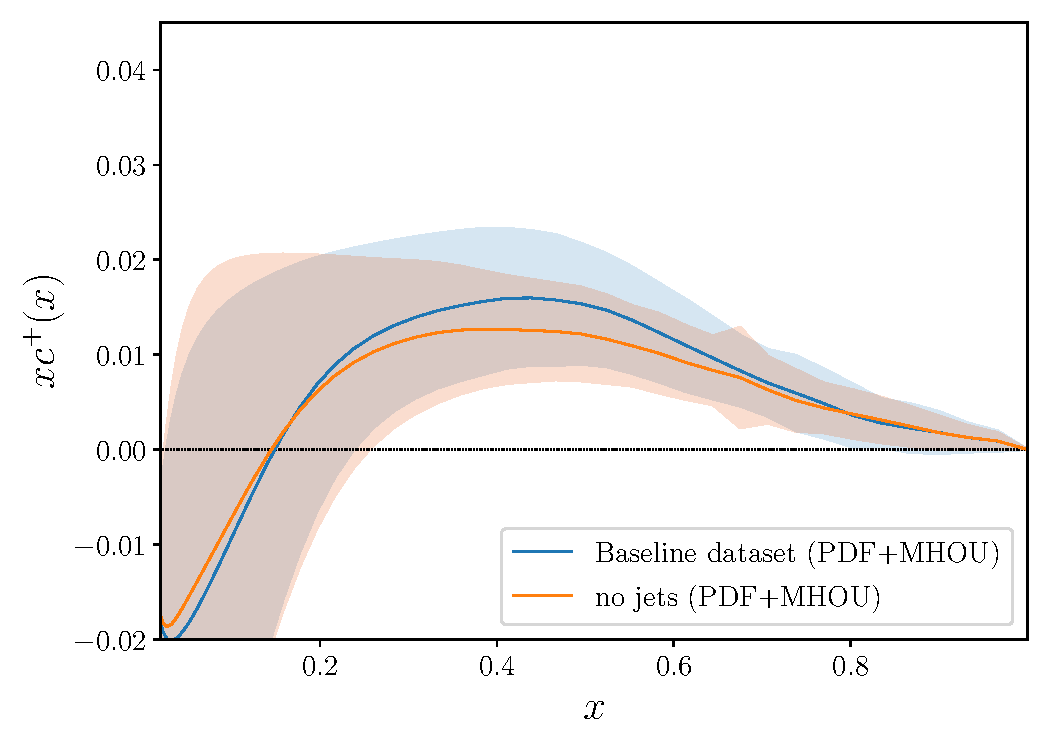
\includegraphics[width=0.49\linewidth]{ch-ic/nojets_Quad_MHOU.pdf}
    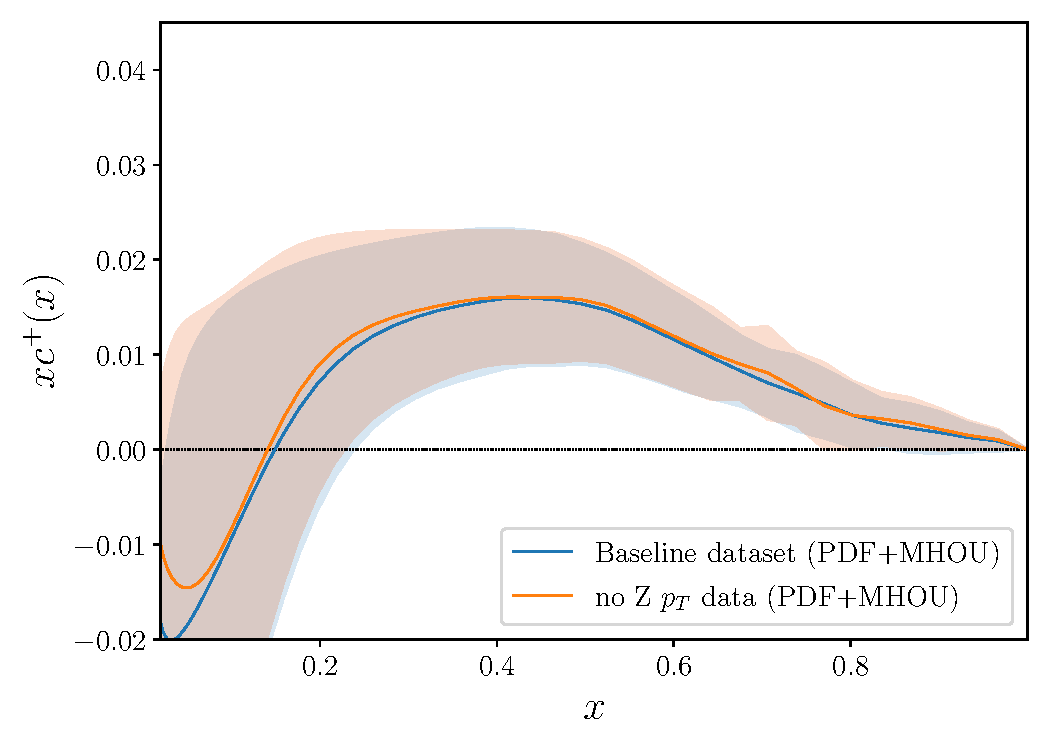
\includegraphics[width=0.49\linewidth]{ch-ic/noZpT_Quad_MHOU.pdf}
    \caption{\small Same as Fig.~\ref{fig:ic/charm_dataset_dep}
      for the intrinsic charm (3FNS) PDF (top four plots), now also including
      four additional dataset variations:  no ATLAS and CMS $W, Z$
      production data   (third row left),
      no jet data (third row right), no $Z$ $p_T$
      measurements (bottom row left), no HERA
      DIS data (bottom row right).
The error band indicates the PDF uncertainties combined in quadrature with the MHOUs.
\label{fig:ic/charm_dataset_dep_nf3} }
\end{center}
\end{figure}
%%%%%%%%%%%%%%%%%%%%%%%%%%%%%%%%%%%%%%%%%%%%%%%%%%%%%%%%%%%%%%%%%%%%%%

We conclude that
the characteristic valence-like peak structure at large-$x$
predicted by non-perturbative intrinsic charm models (Fig.~\ref{fig:ic/charm_content_3fns}
in the main manuscript)
is always present even under very significant changes of the dataset.
%

\paragraph{Dependence on the parametrization basis.}
%
Fig.~\ref{fig:ic/charm_basisdep_3FNS} displays
the comparison between the intrinsic charm
PDF determined with the default evolution basis choice, and the flavor
basis. Complete consistency of central values is found, with somewhat
larger uncertainties in the case of the flavor basis, due to the more 
challenging fitting environment in this basis (see the discussion in~\cite{Ball:2021leu}).

%%%%%%%%%%%%%%%%%%%%%%%%%%%%%%%%%%%%%%%%%%%%%%%%%%%%%%%%%%%%%%%%%%%
\begin{figure}[t!]
  \begin{center}
    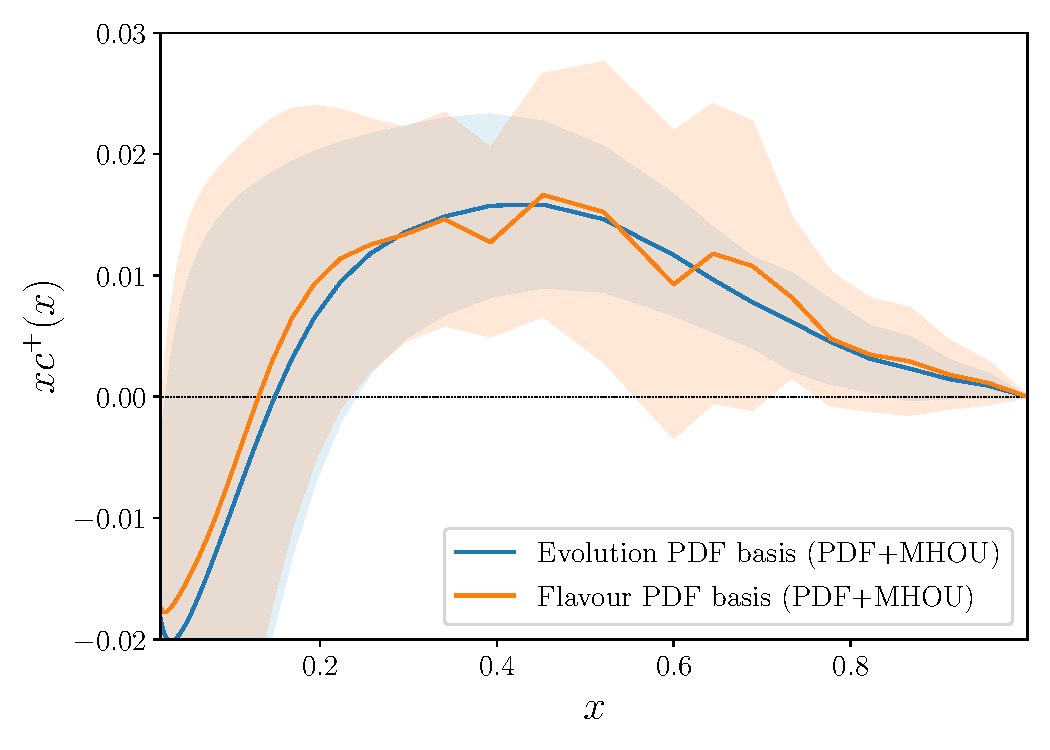
\includegraphics[width=0.54\linewidth]{ch-ic/Flavor_Basis_Quad_MHOU.pdf}
    \caption{\small Same as Fig.~\ref{fig:ic/charm_basisdep}
    for the intrinsic (3FNS) charm.
  \label{fig:ic/charm_basisdep_3FNS} }
\end{center}
\end{figure}
%%%%%%%%%%%%%%%%%%%%%%%%%%%%%%%%%%%%%%%%%%%%%%%%%%%%%%%%%%%%%%%%%%%%%%


\paragraph{Dependence on the charm mass value.}
%
The study of the charm mass dependence is particularly interesting,
because the intrinsic component should be independent of it, hence the
residual dependence seen in Fig.~\ref{fig:ic/charm_fitted_mcdep} in the
4FNS, due to the mass dependence of the perturbative component that
could not be reabsorbed in the fitting, should no longer be present. 
Results are shown in
Fig.~\ref{fig:ic/mass_variations_Quad_MHOU}, and it is apparent that
indeed the dependence on the charm mass has all but disappeared.


%%%%%%%%%%%%%%%%%%%%%%%%%%%%%%%%%%%%%%%%%%%%%%%%%%%%%%%%%%%%%%%%%%%
\begin{figure}[h]
  \begin{center}
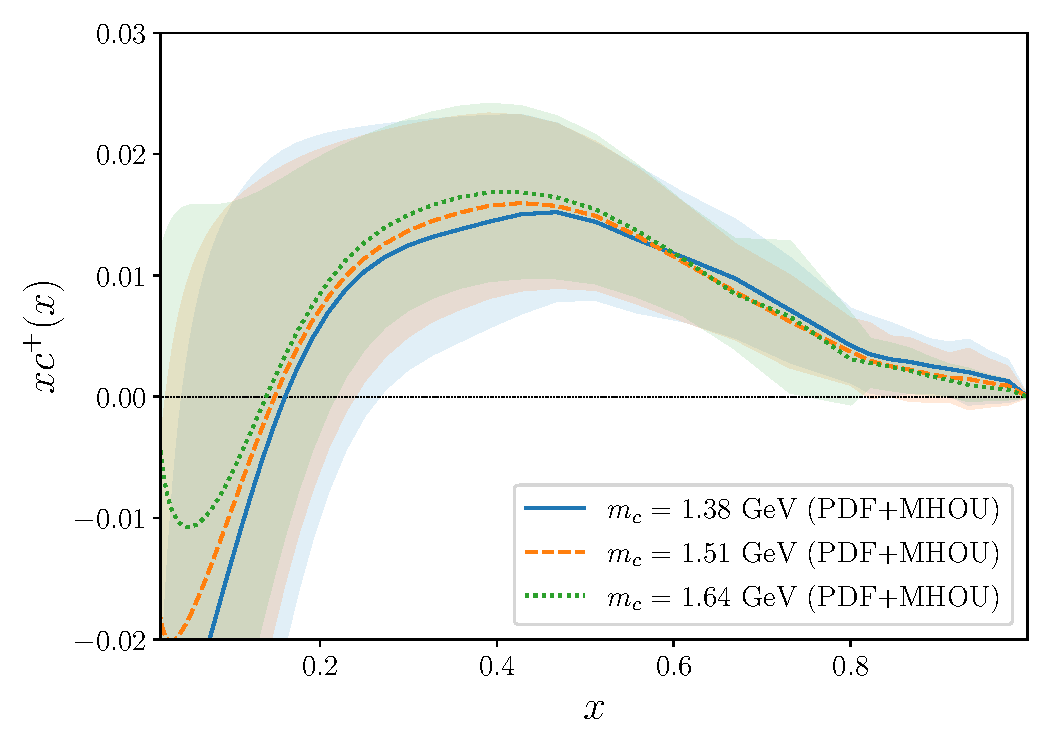
\includegraphics[width=0.49\linewidth]{ch-ic/mass_variations_Quad_MHOU.pdf}
    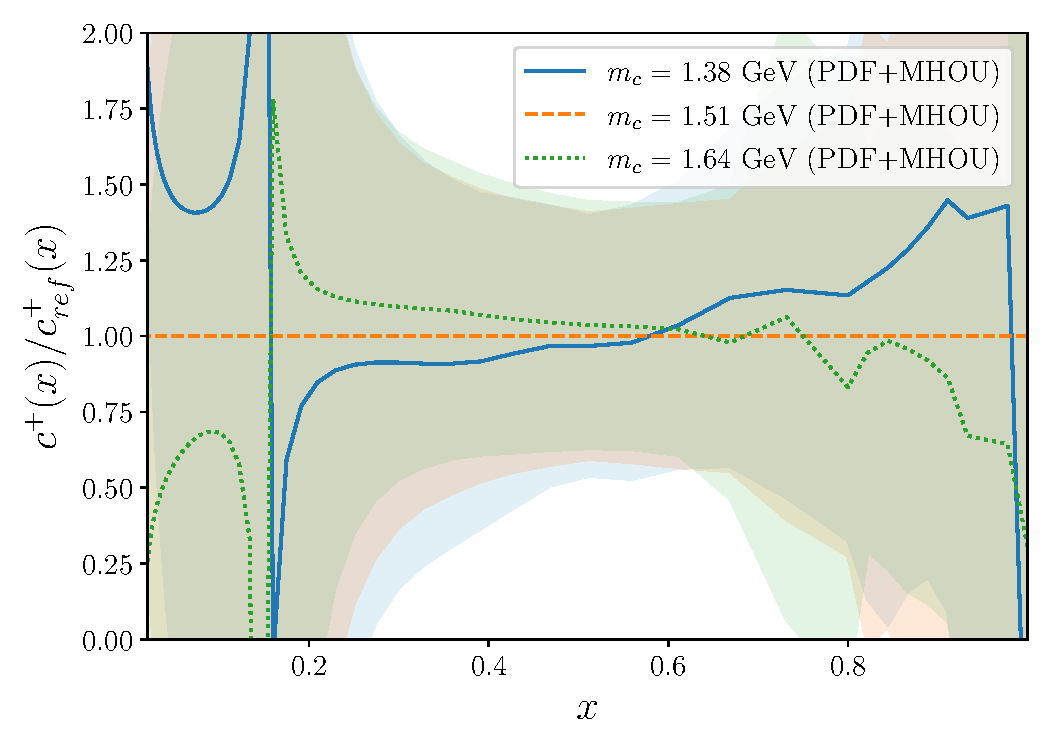
\includegraphics[width=0.49\linewidth]{ch-ic/mass_variations_ratio_Quad_MHOU.pdf}
\caption{\small      
 Same as Fig.~\ref{fig:ic/charm_fitted_mcdep}, now for
      the intrinsic (3FNS) charm PDF. Note that the intrinsic charm
      PDF is scale independent.
  \label{fig:ic/mass_variations_Quad_MHOU} }
\end{center}
\end{figure}
%%%%%%%%%%%%%%%%%%%%%%%%%%%%%%%%%%%%%%%%%%%%%%%%%%%%%%%%%%%%%%%%%%%%%%


\section{The charm momentum fraction}
\label{app:ic/charm_mom_frac}

The fraction of the proton momentum carried by charm quarks
is given by
\begin{equation}
\label{eq:ic/charm_momentum_fraction}
\left[ c\right] = \int_0^1dx\, x c^+(x,Q^2) \, .
\end{equation}
Model predictions, as mentioned, are typically provided up to an
overall normalization, which in turn determines the charm momentum fraction.
%
Consequently, the momentum fraction is often cited as a characteristic
parameter of intrinsic charm.
%
It should however be borne in mind that,
even in the absence of intrinsic charm, this charm momentum fraction is nonzero due
to the perturbative contribution.

In Table~\ref{tab:ic/momfrac_lowQ} we indicate
the values of the charm momentum fraction
 in the 3FNS for our default charm
  determination and in the 4FNS  (at $Q=1.65$ GeV) both for the
  default result and for perturbative charm PDF (see SI Sect.~\ref{app:ic/consistency}).
%
We provide results for  three different values of the charm mass $m_c$ and
indicate separately the PDF and the MHO uncertainties.
%
The 3FNS result is scale-independent, it corresponds to the
momentum fraction carried by intrinsic charm, and it vanishes identically
by assumption in the perturbative charm case.
%
The 4FNS result corresponds to
the scale-dependent momentum fraction that combines the intrinsic and
perturbative contribution, while of course it contains only the
perturbative contribution in the case of perturbative charm.
%
As
discussed in SI Sect.~\ref{app:ic/consistency}, the large uncertainty
associated to higher order corrections to the matching conditions
affects the 3FNS result (intrinsic charm) in the default case, in
which the charm PDF is determined from data in the 4FNS scheme, while
it affects the 4FNS result for perturbative charm, that is determined
assuming the vanishing of the 3FNS result.

 For our default determination, the charm
momentum fraction in the 4FNS at low scale
differs from zero at the $3\sigma$
level.
%
However, it is not possible to tell whether this is of
perturbative or intrinsic origin, because, due to  the large MHOU in
the matching condition, the intrinsic (3FNS) charm momentum fraction
is compatible with zero. This large uncertainty is entirely due to the
small $x\lsim 0.2$ region, see see
Fig.~\ref{fig:ic/charm_content_3fns}~(right).
%
Accordingly, for perturbative charm the
low-scale 4FNS
momentum fraction is compatible with zero.
%
Consistently with the results of SI Sect.~\ref{app:ic/charm_stability_4fns},
the 4FNS result is essentially independent of the value of the charm
mass, but it becomes strongly dependent on it if one assumes
perturbative charm.

%%%%%%%%%%%%%%%%%%%%%%%%%%%%%%%%%%%%%%%%%%%%%%%%%%%%%%%%%%%%%%%%%%%%%%%%%%%%%%%
\begin{table}[t]
  \footnotesize
  \centering
    \renewcommand{\arraystretch}{1.30}
\begin{tabularx}{\textwidth}{C{2.0cm}C{2.3cm}C{2.2cm}C{2.2cm}C{5.6cm}}
  \toprule
  Scheme  & $Q$ & Charm PDF & $m_c$  &  $\left[ c\right]~\left(\%\right)$ \\
  \midrule
  \midrule
 3FNS  & --  &default  &  1.51 GeV  &   $ 0.62\pm0.28_\textrm{ pdf}\pm 0.54_\textrm{ mhou} $ \\
 3FNS  & --  &default  &  1.38 GeV  &   $ 0.47\pm0.27_\textrm{ pdf}\pm 0.62_\textrm{ mhou} $ \\
 3FNS  & --  &default  &  1.64 GeV  &    $ 0.77\pm0.28_\textrm{
  pdf}\pm 0.48_\textrm{ mhou} $ \\
  \midrule

 4FNS  & 1.65 GeV  & default  &  1.51 GeV  &   $0.87 \pm 0.23_\textrm{ pdf}$  \\
 4FNS  & 1.65 GeV  & default &  1.38 GeV  &   $0.94 \pm 0.22_\textrm{ pdf}$  \\
 4FNS  & 1.65 GeV  & default   &  1.64 GeV  &  $0.84 \pm 0.24_\textrm{ pdf}$  \\
  \midrule
 \midrule
 4FNS  & 1.65 GeV   & perturbative  &  1.51 GeV  &   $0.346\pm 0.005_\textrm{ pdf}\pm 0.44_\textrm{ mhou}$ \\
 4FNS  & 1.65 GeV   & perturbative  &  1.38 GeV  &    $0.536\pm 0.006_\textrm{ pdf}\pm 0.49_\textrm{ mhou}$ \\
 4FNS  & 1.65 GeV   & perturbative  &  1.64 GeV  &    $0.172\pm 0.003_\textrm{ pdf}\pm 0.41_\textrm{ mhou}$ \\
\bottomrule
\end{tabularx}
\vspace{0.3cm}
\caption{\label{tab:ic/momfrac_lowQ}
  The charm momentum fraction, Eq.~(\ref{eq:ic/charm_momentum_fraction}).
  %
  We show  results both in the 3FNS and the 4FNS (at $Q=1.65$ GeV)
  for our default charm, and also in the 4FNS for perturbative charm.
  %
We provide results for  three different values of the charm mass $m_c$ and
indicate separately the PDF and the MHO uncertainties.
}
\end{table}
%%%%%%%%%%%%%%%%%%%%%%%%%%%%%%%%%%%%%%%%%%%%%%%%%%%%%%%%%%%%%%%%%%%%%%%%%%%%%%%

%%%%%%%%%%%%%%%%%%%%%%%%%%%%%%%%%%%%%%%%%%%%%%%%%%%%%%%%%%%%%%%%%%%
\begin{figure}[h]
  \begin{center}
     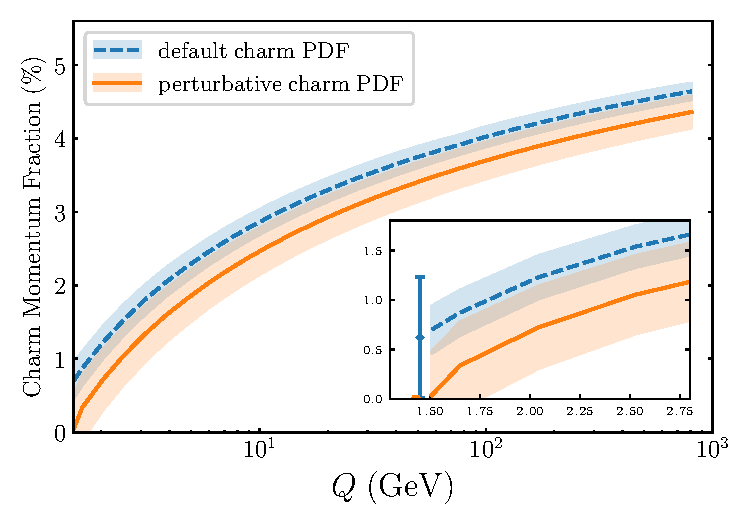
\includegraphics[width=0.60\linewidth]{ch-ic/charm_momfrac_qdep.pdf}
    \caption{\small 
      The 4FNS charm momentum fraction in NNPDF4.0 as a function of scale $Q$,
      both for the default and perturbative charm cases,
      for a charm mass value of $m_c=1.51$ GeV.
      %
     The inset zooms on the low-$Q$ region and includes the 3FNS
     (default) result
     from Table~\ref{tab:ic/momfrac_lowQ}. 
     %
     Note that the uncertainty includes the MHOU for the 3FNS default
     and 4FNS perturbative charm cases, while it is the PDF
     uncertainty for the 4FNS default charm case.
  \label{fig:ic/comparison_IC_models} }
\end{center}
\end{figure}
%%%%%%%%%%%%%%%%%%%%%%%%%%%%%%%%%%%%%%%%%%%%%%%%%%%%%%%%%%%%%%%%%%%%%%

The 4FNS charm momentum fraction is plotted as a function of scale
in Fig.~\ref{fig:ic/comparison_IC_models}, both in the default case and
for perturbative charm, with the 3FNS values and the detail of the low-$Q$ 
4FNS results shown in an inset.
%
The dependence on the value of the charm mass
is shown in Fig.~\ref{fig:ic/charm_momfrac_qdep_mc}.
The large MHOUs on the 3FNS result, and on the 
4FNS result in the case of perturbative charm, are apparent.
The stability of the default result upon variation of  the value of
$m_c$, and the strong dependence of the perturbative charm result on
$m_c$, are  also clear.
Both the large MHOU uncertainty, and the strong dependence on
the value of $m_c$
for perturbative charm are seen to persist up to large scales.


%%%%%%%%%%%%%%%%%%%%%%%%%%%%%%%%%%%%%%%%%%%%%%%%%%%%%%%%%%%%%%%%%%%
\begin{figure}[t]
  \begin{center}
    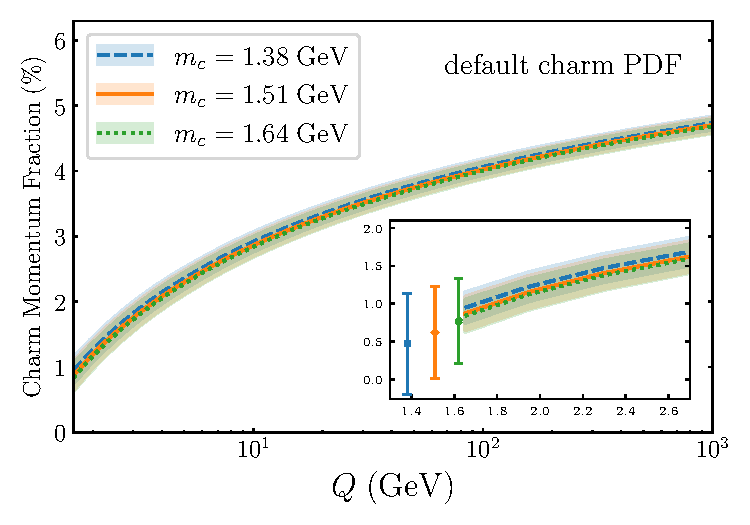
\includegraphics[width=0.49\linewidth]{ch-ic/charm_momfrac_qdep_mc.pdf}
    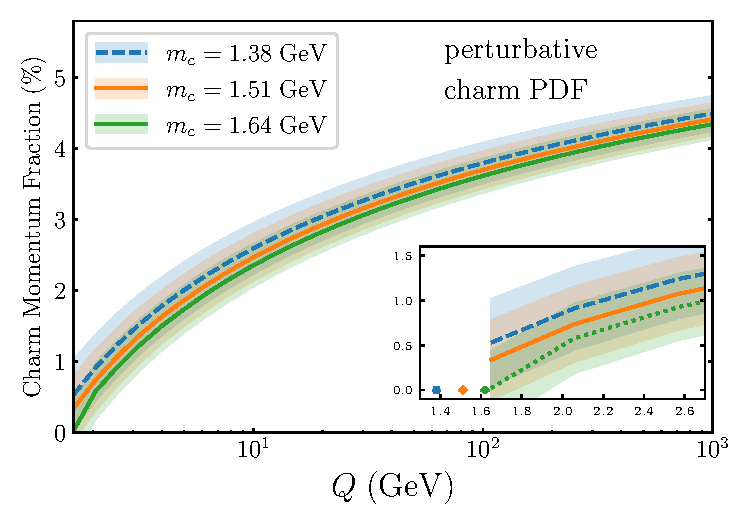
\includegraphics[width=0.49\linewidth]{ch-ic/charm_momfrac_qdep_mc_pert.pdf}
    \caption{\small
    Same as Fig.~\ref{fig:ic/comparison_IC_models} for different values
    of the charm mass. Note that the 3FNS momentum fraction for
     perturbative charm vanishes identically by assumption.
   \label{fig:ic/charm_momfrac_qdep_mc} }
\end{center}
\end{figure}
%%%%%%%%%%%%%%%%%%%%%%%%%%%%%%%%%%%%%%%%%%%%%%%%%%%%%%%%%%%%%%%%%

It is interesting to understand in detail the impact of the MHOU on
the momentum fraction carried by intrinsic charm. To this purpose, we
have computed  the truncated momentum integral, i.e. 
  Eq.~(\ref{eq:ic/charm_momentum_fraction}) but only integrated down to
  some  lower
  integration limit $x_\textrm{ min}$:
  \begin{equation}
\label{eq:ic/charm_momentum_fraction_truncated}
\left[ c\right]_\textrm{ tr}(x_\textrm{ min}) \equiv \int_{x_\textrm{ min}}^1dx\, x c^+(x,Q^2) \, .
\end{equation}
Note than in the 3FNS   $x
c^+(x)$ does not depend on scale, so  this becomes
a scale-independent quantity.
%
The result for our default intrinsic charm determination is displayed
in Fig.~\ref{fig:ic/charm_momfrac_xmin_dep}, as a function of
of the lower integration limit $x_\textrm{ min}$.
%
It is clear that for $x_\textrm{ min} \gtrsim 0.2$ the truncated momentum
fraction  differs significantly from zero, thereby providing evidence
for intrinsic charm with similar statistical  significance as the
local pull shown in Fig.~\ref{fig:ic/Zc} bottom left.
%
For $x \lsim 0.2$
this  significance is then washed out
by the large MHOUs.

Hence, while the total momentum fraction has been traditionally adopted
as a measure of intrinsic charm, 
our analysis shows that, once MHOUs are accounted for, the information
provided by the total momentum fraction is limited, at least with
current data and theory.



%%%%%%%%%%%%%%%%%%%%%%%%%%%%%%%%%%%%%%%%%%%%%%%%%%%%%%%%%%%%%%%%%%%
\begin{figure}[h!]
  \begin{center}
    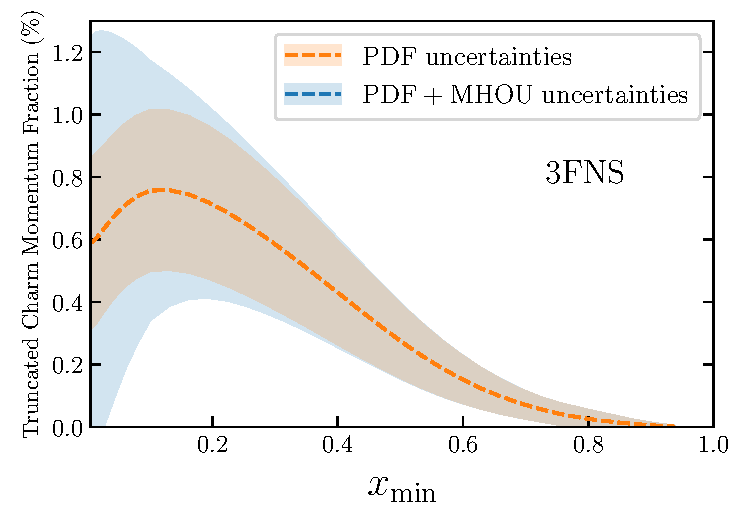
\includegraphics[width=0.65\linewidth]{ch-ic/charm_momfrac_xmin_dep_3fns.pdf}
    \caption{\small The value of the truncated charm momentum integral,
      Eq.~(\ref{eq:ic/charm_momentum_fraction_truncated}), as a function
      of the lower integration limit $x_\textrm{ min}$
      for our baseline determination of the 3FNS intrinsic charm PDF.
      %
      We display separately the PDF and the total (PDF+MHOU) uncertainties.
  \label{fig:ic/charm_momfrac_xmin_dep} }
\end{center}
\end{figure}
%%%%%%%%%%%%%%%%%%%%%%%%%%%%%%%%%%%%%%%%%%%%%%%%%%%%%%%%%%%%%%%%%%%%%%



\section{Comparison with  CT14IC}
\label{app:ic/ct}

The possibility of an intrinsic charm component was recently studied
in~\cite{Hou:2017khm}, by modifying the CT14 PDF set, with the
initial 4FNS charm PDF taken equal to the BHPS
model~\cite{Brodsky:1980pb} form with the normalization fitted as a
free parameter.
%
A 4FNS  charm PDF with uncertainties at $Q=1.3$~GeV was then
constructed by taking 
the BHPS model with best-fit normalization as central value (called
the `BHPS1 model' in~\cite{Hou:2017khm}); the lower
edge of the uncertainty band was taken to coincide with the standard
CT14 charm PDF  (i.e. the charm PDF determined by perturbative
matching from the 3FNS to the 4FNS); the upper edge of the uncertainty
band was taken as 
the BHPS model but with  normalization fixed to the upper  90\% CL limit (called the
`BHPS2 model' in~\cite{Hou:2017khm}).

%%%%%%%%%%%%%%%%%%%%%%%%%%%%%%%%%%%%%%%%%%%%%%%%%%%%%%%%%%%%%%%%%%%
\begin{figure}[h]
  \begin{center}
    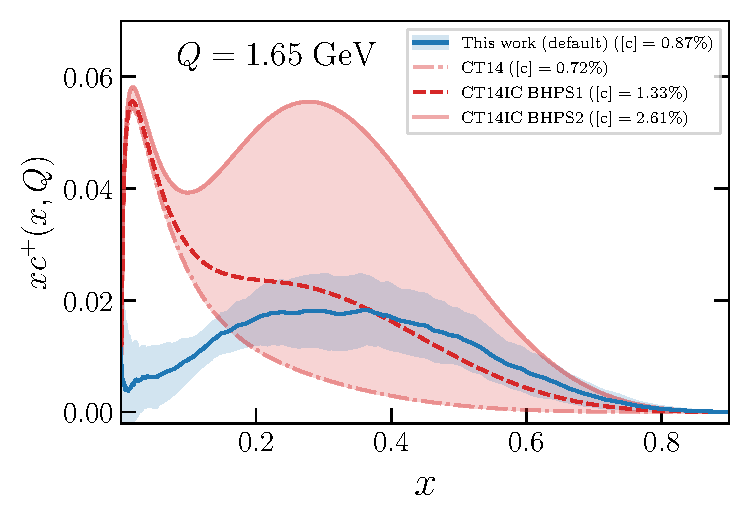
\includegraphics[width=0.49\linewidth]{ch-ic/pdfplot-abs-lin-charm-q1p65gev.pdf}
    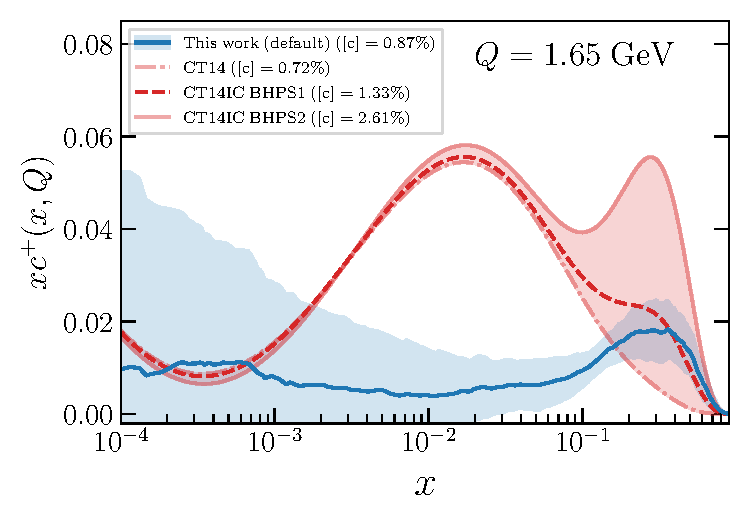
\includegraphics[width=0.49\linewidth]{ch-ic/pdfplot-abscharm-q1p65gev.pdf}
    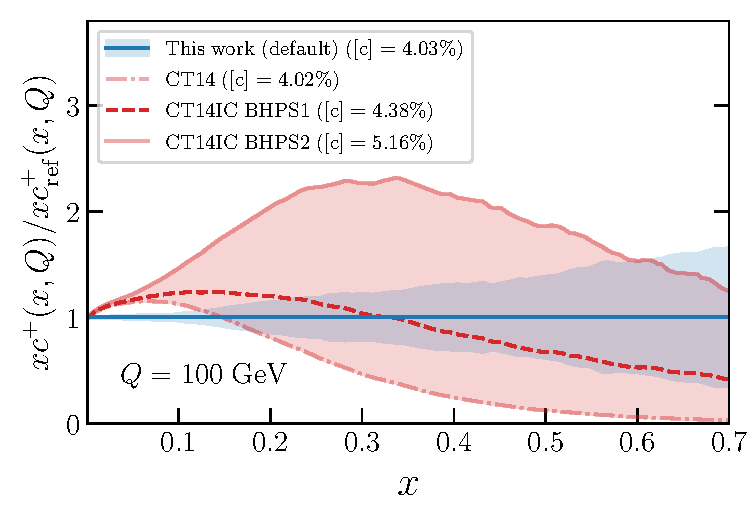
\includegraphics[width=0.49\linewidth]{ch-ic/pdfplot-abscharm-q100gev.pdf}	
    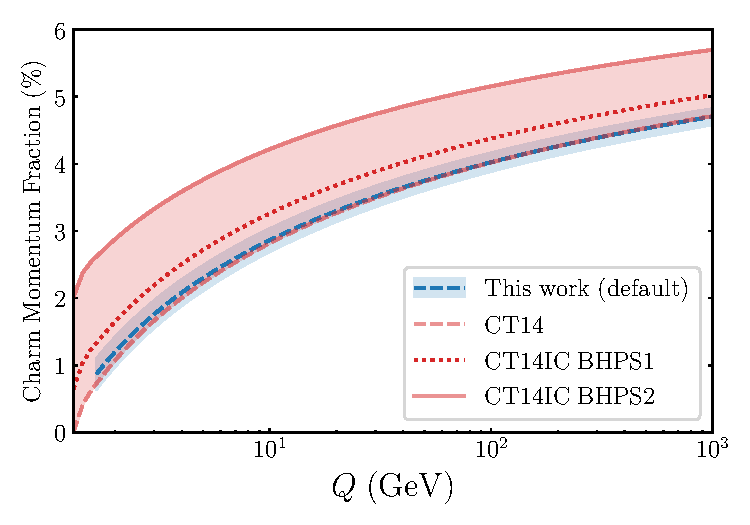
\includegraphics[width=0.49\linewidth]{ch-ic/charm_momfrac_qdep_ct.pdf}
    \caption{\small The 4FNS charm PDF
    from~\cite{Hou:2017khm} compared to our result (also in the 4FNS) 
     at $Q=1.65$~GeV on
    a linear (top left) and logarithmic (top right) scale in $x$, and
    at  $Q=100$~GeV on a linear scale in $x$ and as a ratio to our result
    (bottom left).
    %
    The momentum fraction corresponding to either case
    is also shown as a function of $Q$ (bottom right). Note that for
    our result the uncertainty band is the 68\%CL PDF uncertainty,
    while for~\cite{Hou:2017khm} the central curve (labeled
    CT14IC BHPS1) corresponds to the BHPS model with best-fit
    normalization, the lower curve (labeled
    CT14) corresponds to the default CT14 perturbative charm PDF and
    the upper curve (labeled
    CT14IC BHPS2) corresponds to the BHPS model with normalization at
    the upper 90\% CL (see text). The value of the momentum fractions
    are also provided in each case.
  \label{fig:ic/comparison_CT14} }
\end{center}
\end{figure}
%%%%%%%%%%%%%%%%%%%%%%%%%%%%%%%%%%%%%%%%%%%%%%%%%%%%%%%%%%%%%%%%%%%%%%

The CT14IC charm PDF is compared to our result in
Fig.~\ref{fig:ic/comparison_CT14}, at  $Q=1.65$ GeV and $Q=100$ GeV, in
the former case on both a logarithmic and linear scale in $x$ and in
the latter case on a linear scale only, as a ratio to our default
result.
%
Note that the uncertainty band has a different interpretation in the
two curves shown: for our result it is the 68\%~CL PDF uncertainty,
while for~\cite{Hou:2017khm}  it corresponds to the model
uncertainty estimated as described above.
%
In Fig.~\ref{fig:ic/comparison_CT14} we also quote
the charm momentum fraction in each case, at the corresponding scale $Q$. 

As shown in Fig.~\ref{fig:ic/charm_content_3fns} (right), our result for
the charm PDF is in good agreement with the BHPS model at large
$x$. Correspondingly, for $x\gsim 0.3$
we find reasonably good agreement between our
result and the central curve of~\cite{Hou:2017khm}, which
corresponds to a momentum fraction and thus a normalization of the charm
PDF not too different from our result (see Table~\ref{tab:ic/momfrac_lowQ}).
%
Both the upper and lower curve from~\cite{Hou:2017khm} instead
do not agree with our result within uncertainties: indeed the
lower edge corresponds to the absence of intrinsic charm (which we
exclude) and the upper edge to a momentum fraction which we exclude
at more than the $5\sigma$ level (see Table~\ref{tab:ic/momfrac_lowQ}). 

For intermediate values $3\cdot10^{-3}\lsim x\lsim 0.3$  our result disagrees
with that of 
~\cite{Hou:2017khm}, while at very small $x$ all results agree,
the intrinsic charm being compatible with zero.
The disagreement at intermediate $x$ is mostly due
to the fact that in ~\cite{Hou:2017khm} charm is assumed to take
the BHPS form, which vanishes for $x\lsim 0.1$,
in the 4FNS at the low scale $Q=1.3$~GeV.
%
Due to perturbative evolution from  $Q=1.3$~GeV to $Q=1.65$~GeV the charm 
PDF then develops the large bump that is
seen in Fig.~\ref{fig:ic/comparison_CT14}, where we instead find that 
the 4FNS charm PDF is quite small.
%
This difference persists at large scales as seen  in
Fig.~\ref{fig:ic/charm_content_3fns} (bottom left).

In terms of momentum fractions, shown in Fig.~\ref{fig:ic/charm_content_3fns} (bottom right),
as already mentioned our result is
compatible with the central value of~\cite{Hou:2017khm} within
uncertainties; and also with the lower edge of ~\cite{Hou:2017khm}
that corresponds to perturbative charm.
%
The upper edge  of the prediction from~\cite{Hou:2017khm} is instead
ruled out at more than $5\sigma$. 


\section{$Z$+charm production in the forward region}
\label{sec:ic/zcharm}

Here we provide full details on our computation of  $Z$+charm
production and on the inclusion of the LHCb data for this
process in the determination of the charm PDF shown in
Fig.~\ref{fig:ic/Zc}. 

\paragraph{Computational settings.}
%
Theoretical predictions for
the $Z$+charm measurements in the forward region 
by LHCb~\cite{LHCb:2021stx} follow the 
 settings described in~\cite{Boettcher:2015sqn}.
%
$Z$+jet events at NLO QCD theory are generated for $\sqrt{s}= 13$ TeV  using the $Zj$ package of the
\textsc{\small POWHEG-BOX}~\cite{Alioli:2010xd}.
%
The parton-level events produced by \textsc{\small POWHEG}
are then interfaced to \textsc{\small Pythia8}~\cite{Sjostrand:2007gs}
with the Monash 2013 tune~\cite{Skands:2014pea} for showering,
hadronization, and simulation of the underlying event and multiple
parton interactions.
%
Long-lived hadrons, including charmed hadrons,
are assumed stable and not decayed.

Selection criteria on these particle-level events are imposed
to match the LHCb acceptance~\cite{LHCb:2021stx}.
%
$Z$ bosons are reconstructed in the dimuon final state by
requiring $60~\textrm{ GeV}\le m_{\mu\mu} \le 120~\textrm{ GeV}$,
and
only events where these muons satisfy
    $p_T^\mu \ge 20~\textrm{ GeV}$ and $2.0 \le \eta_{\mu}\le 4.5$
    are retained.
%
Stable visible hadrons within the LHCb acceptance of
$2.0 \le \eta \le 4.5$ are clustered with
the anti-$k_T$ algorithm with radius parameter
of $R=0.5$~\cite{Cacciari:2008gp}.
%
Only events with a hardest jet satisfying
  $ 20~\textrm{ GeV} \le p_T^\textrm{ jet} \le 100~\textrm{ GeV}$
and $2.2 \le \eta_\textrm{ jet}\le 4.2$ are retained.
%
Charm jets are defined as jets containing
a charmed hadron, specifically  jets satisfying
$\Delta R(j, c\textrm{-hadron})\le 0.5$ for a charmed
hadron with $p_T(c\textrm{-hadron})\ge 5~\textrm{ GeV}$.
%
Jets and muons are required to be separated
in rapidity and azimuthal angle, so
we require $\Delta R(j, \mu)\ge 0.5$.
%
The resulting events
are then binned in the $Z$ bosom rapidity $y_Z = y_{\mu \mu}$.

The physical observable measured by LHCb is the ratio of the fraction of $Z$+jet
    events with and without a charm tag,
    \begin{equation}
    \label{eq:ic/Rcj}
        \mathcal{R}_j^c \equiv \frac{\sigma(pp\to Z+\textrm{ charm~ jet})}{\sigma(pp \to Z+\textrm{ jet})}=
         \frac{N(c\textrm{ -tag})}{ 
        N(\textrm{ jets})} \, .
    \end{equation}
 Here  $N(c\textrm{ -tag})$ and $N(\textrm{ jets})$ are, respectively, the number
    of charm-tagged and un-tagged jets, for a  $Z$ boson rapidity interval
    that satisfies the selection and acceptance criteria.
    %
    The denominator of Eq.~(\ref{eq:ic/Rcj}) includes all jets, even those
    containing heavy hadrons.
    %
The charm tagging efficiency is already accounted for at the level
of the experimental measurement, so it is not required in the theory
simulations.

Predictions for Eq.~(\ref{eq:ic/Rcj}) are produced using our default PDF
determination (NNPDF4.0 NNLO), as well as the corresponding PDF set
with perturbative charm (see SI Sect.~\ref{app:ic/consistency}).
%
We have
explicitly checked that our results are essentially independent of the
value of the charm mass.
%
We have evaluated MHOUs and PDF uncertainties using the
output of the \textsc{\small POWHEG+Pythia8} calculations.
We have checked that MHOUs, evaluated with the standard
seven-point prescription, essentially cancel in the ratio
Eq.~(\ref{eq:ic/Rcj}). Note that 
this is not the case for  PDF uncertainties, because the dominant
partonic subchannels in the numerator and denominator are not the same.

\paragraph{Inclusion of the LHCb data.}

%%%%%%%%%%%%%%%%%%%%%%%%%%%%%%%%%%%%%%%%%%%%%%%%%%%%%%%%%%%%%%%%%%%%%%%%%%%%%%%
\begin{table}[h]
  \small
    \renewcommand{\arraystretch}{1.45}
\begin{tabularx}{\textwidth}{C{3.5cm}C{2.5cm}C{2.5cm}C{2.5cm}C{2.5cm}}
  \toprule
 \multirow{2}{*}{ $\chi^2/N_\textrm{ dat}$}  &   \multicolumn{2}{c}{ default charm}   &\multicolumn{2}{c}{perturbative charm} \\
                       &  $\rho_\textrm{ sys}=0$   & $\rho_\textrm{ sys}=1$ &  $\rho_\textrm{ sys}=0$ &   $\rho_\textrm{ sys}=1$ \\
  \midrule
 Prior        &  1.85   &  3.33      &   3.54  & 3.85      \\
 \midrule
 Reweighted   &  1.81   &  3.14      &   $-$   &  $-$     \\
\bottomrule
\end{tabularx}
\vspace{0.3cm}
\caption{\label{tab:ic/chi2_zcharm} The values of $\chi^2/N_\textrm{ dat}$
 for the LHCb $Z$+charm data before (prior) and after (reweighted)
 their inclusion in the PDF fit. Results are given for two 
 experimental correlation models, denoted as
 $\rho_\textrm{ sys}=0$ and $\rho_\textrm{ sys}=1$. We also report values
 before inclusion for the perturbative charm PDFs.
}
\end{table}
%%%%%%%%%%%%%%%%%%%%%%%%%%%%%%%%%%%%%%%%%%%%%%%%%%%%%%%%%%%%%%%%%%%%%%%%%%%%%%%

We first compare the quality of the description of the LHCb data
before their inclusion. In Table~\ref{tab:ic/chi2_zcharm} we show the
values of $\chi^2/N_\textrm{ dat}$ for the LHCb $Z$+charm data
both with default and perturbative charm.
%
Since the experimental covariance matrix is not available for the LHCb
data we determine the $\chi^2$ values assuming two limiting scenarios
for the correlation of experimental systematic uncertainties.
%
Namely, 
we either add in quadrature statistical and systematic errors ($\rho_\textrm{ sys}=0$),
or alternatively we assume that the total systematic uncertainty
is fully correlated between $y_Z$ bins ($\rho_\textrm{ sys}=1$). Fit
quality is always significantly better in our default intrinsic charm
scenario than with perturbative charm.
%
As is clear from
Fig.~\ref{fig:ic/Zc} (top left), the somewhat poor fit quality is mostly due to the first
rapidity bin, which is essentially uncorrelated to the amount of
intrinsic charm (see
Fig.~\ref{fig:ic/Zc}, top right).

The LHCb $Z$+charm data are then included in the PDF determination
through
Bayesian reweighting~\cite{Ball:2010gb,Ball:2011gg}. The
$\chi^2/N_\textrm{ dat}$ values obtained using the PDFs found after their
inclusion are given in
Table~\ref{tab:ic/chi2_zcharm}.
%
They are computed by combining the PDF and
experimental covariance matrix so both sources of uncertainty are
included --- as mentioned above, MHOUs are negligible.
The fit quality is seen to improve only
mildly, and the effective number of
replicas~\cite{Ball:2010gb,Ball:2011gg} after reweighting
is only moderately reduced, from the prior $N_\textrm{ rep}=100$ to $N_\textrm{
eff}=92$ or $N_\textrm{ eff}=84$ in the
$\rho_\textrm{ sys}=0$ and $\rho_\textrm{ sys}=1$ scenarios respectively.
%
This
demonstrates that the inclusion of the LHCb $Z$+charm measurements  affects
the PDFs only weakly. This agrees with the results shown in 
Figs.~\ref{fig:ic/Zc}~(center) in
the main manuscript, where it is seen that the inclusion of the LHCb
data has essentially no impact on the shape of the charm PDF, but
it moderately reduces its uncertainty in the region of the valence peak.



\section{Parton luminosities}
\label{sec:ic/lumis}

The impact of intrinsic charm on hadron collider observables can be
assessed by studying  parton luminosities. Indeed, the
cross-section for hadronic processes at leading order is typically
proportional to an individual parton luminosity or linear combination
of parton luminosities.
%
Comparing parton luminosities determined
using our default PDF set to those obtained imposing perturbative
charm (see SI Sect.~\ref{app:ic/consistency}) provides a qualitative estimate of the
measurable impact of intrinsic charm. Of course this is then modified
by higher-order
perturbative corrections, which generally depend on more partonic
subchannels and thus on more luminosities.
%
In this section we illustrate this by considering the parton
luminosities that are relevant for the computation of the
$Z$+charm process in the LHCb kinematics, see SI Sect.~\ref{sec:ic/zcharm}.

The parton luminosity without any restriction on the rapidity $y_X$ of the final state is
\begin{equation}
\label{eq:ic/lumi1D}
\mathcal{L}_{ab}(m_X)= \frac{1}{s}\int_{\tau}^1 \frac{dx}{x}f_a \left( x,m_X^2\right)
f_b\left( \tau/x,m_X^2\right) \, ,\qquad
\tau=\frac{m_X^2}{s} \, ,
\end{equation}
where $a,b$ label the species of incoming partons, $\sqrt{s}$ is the center-of-mass energy of
the hadronic collision, and $m_X$ is the final state invariant mass.
%
For the more realistic situation where the final state rapidity
is restricted, $y_\textrm{ min}\le y_X\le y_\textrm{ max}$,
Eq.~(\ref{eq:ic/lumi1D}) is modified as
\begin{equation}
\label{eq:ic/lumi1D_restricted}
\mathcal{L}_{ab}(m_X)= \frac{1}{s}\int_{\tau}^1 \frac{dx}{x}f_a \left( x,m_X^2\right)
f_b\left( \tau/x,m_X^2\right) \theta\left( y_X-y_\textrm{ min}  \right)
\theta\left( y_\textrm{ max}-y_X  \right)\, , 
\end{equation}
where $y_X = \left( \ln x^2/\tau \right) /2$.

We consider in particular the quark-gluon and the charm-gluon luminosities, defined as
\begin{equation}
\label{eq:ic/lumis}
\mathcal{L}_{qg}(m_X)\equiv \sum_{i=1}^{n_f} \left( \mathcal{L}_{q_ig}(m_X)+
\mathcal{L}_{\bar{q}_ig}(m_X) \right)\, , \quad
\mathcal{L}_{cg}(m_X)\equiv  \left( \mathcal{L}_{cg}(m_X)+
\mathcal{L}_{\bar{c}g}(m_X) \right)\, , 
\end{equation}
where $n_f$ is the number of active quark flavors for a given value of $Q=m_X$
with a maximum value of $n_f=5$.
%
These are the combinations that provide the leading contributions
respectively to the numerator ($\mathcal{L}_{cg}$) and the 
denominator
($\mathcal{L}_{qg}$) of  $\mathcal{R}_j^c$ in Eq.~(\ref{eq:ic/Rcj}). 

%%%%%%%%%%%%%%%%%%%%%%%%%%%%%%%%%%%%%%%%%%%%%%%%%%%%%%%%%%%%%%%%%%%
\begin{figure}[htbp]
  \begin{center}
    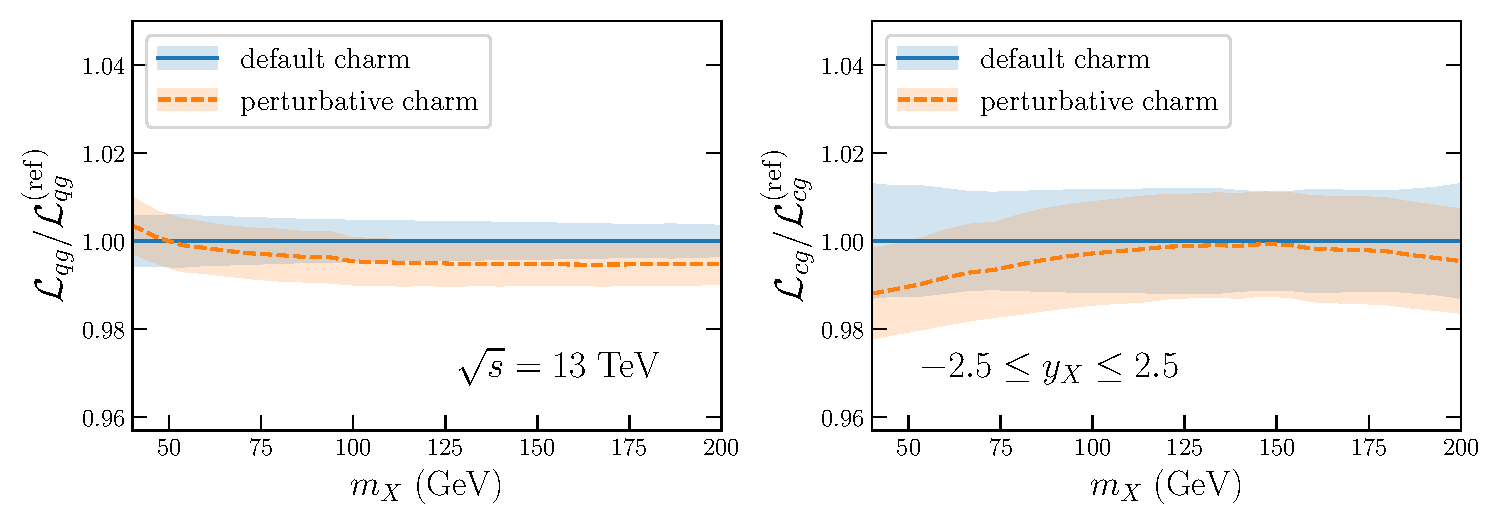
\includegraphics[width=0.99\linewidth]{ch-ic/cglumi-nnpdf40-ATLAScuts.pdf}
    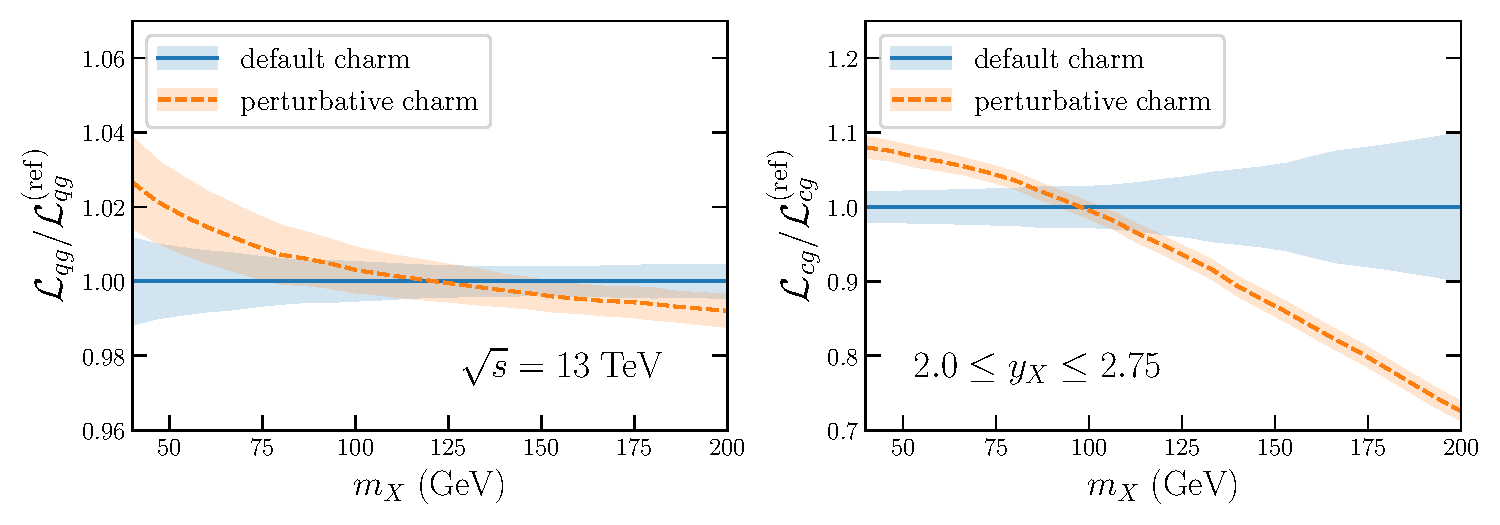
\includegraphics[width=0.99\linewidth]{ch-ic/cglumi-nnpdf40-LHCbcuts-central.pdf}
    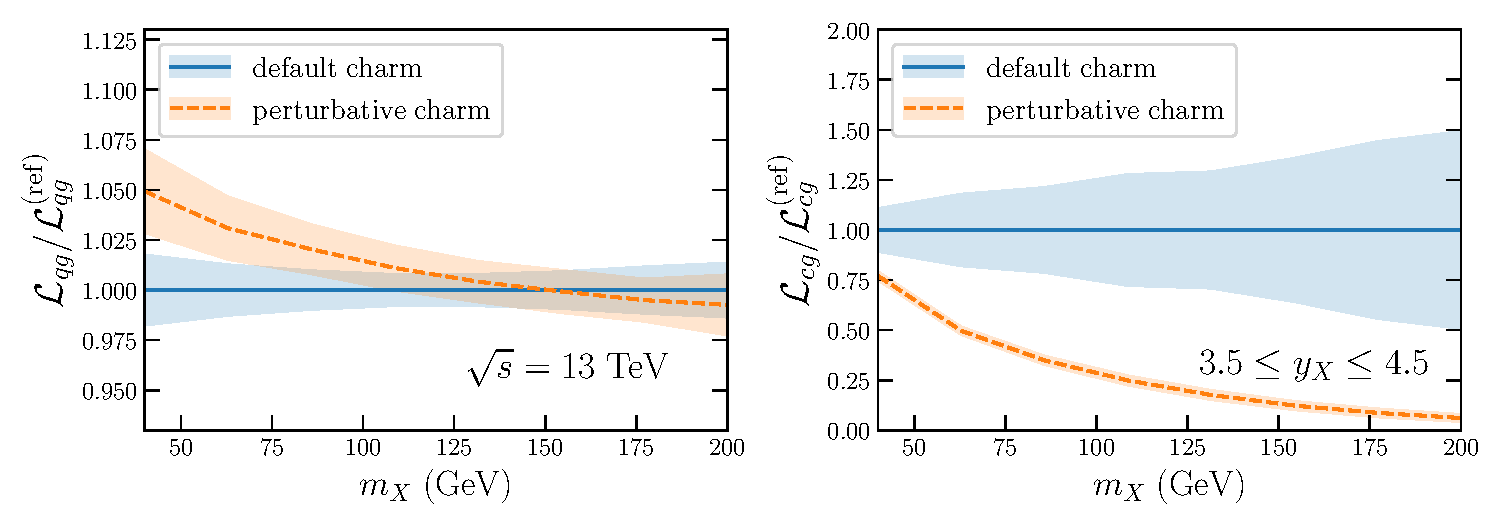
\includegraphics[width=0.99\linewidth]{ch-ic/cglumi-nnpdf40-LHCbcuts-forward.pdf}
    \caption{\small The quark-gluon (left) and charm-gluon (right)
      parton luminosities in the  $m_X$ region
      relevant for $Z$+charm production and  three different
      rapidity bins (see text). Results are shown both for our default charm
    PDFs and for the variant with perturbative charm. 
  \label{fig:ic/charm_luminosities} }
\end{center}
\end{figure}
%%%%%%%%%%%%%%%%%%%%%%%%%%%%%%%%%%%%%%%%%%%%%%%%%%%%%%%%%%%%%%%%%

The luminosities are displayed in Fig.~\ref{fig:ic/charm_luminosities},
in the  invariant mass region,
$40~\textrm{ GeV}\le m_X \le 200~\textrm{ GeV}$ which is most relevant for
$Z$+charm production.
%
Results are shown 
for three different
rapidity bins, $-2.5 \le y_X \le 2.5$ (central production in ATLAS and CMS),
$2.0 \le y_X \le 2.75$ (forward production, corresponding to the
central bin in LHCb),
and $3.5 \le y_X \le 4.5$ (highly boosted production, corresponding to
the most forward bin in the LHCb selection), as a ratio to our default case.

For central production it is clear that both the quark-gluon and
charm-gluon luminosities with our without intrinsic charm are very similar.
This means that central $Z$+charm production in this invariant mass
range is insensitive to intrinsic charm.
%
For forward production, corresponding to the  central LHCb rapidity
bin, $2.0 \le y_X \le 2.75$, in the invariant mass region  $m_X\simeq
100$~GeV again there is little difference between results with or
without intrinsic charm, but as the invariant mass increases the
charm-gluon luminosity with intrinsic charm is significantly enhanced.
%
For very forward production, such as the highest rapidity bin of LHCb,
$3.5 \le y_X \le 4.5$, the charm-gluon luminosity 
at $m_X \simeq 100$ GeV is enhanced  by a factor of about 4 in our
default result in comparison to the perturbative charm case, corresponding
to a $\simeq 3\sigma$ difference in units of the PDF uncertainty,
consistently with the behavior observed for the 
$\mathcal{R}_j^c$ observable in Fig.~\ref{fig:ic/Zc}~(top left) in the
most forward rapidity  bin.
%
This observation provides a qualitative explanation of
the results of SI Sect.~\ref{sec:ic/zcharm}.
